% =============================================================================
%  Week 1 briefing -- metamemory in streaming egocentric video-LLMs
%
%  Built by modules, along the same verifiable-artifact boundaries the
%  experiments use.  See README.md for the module map.  Build with `make`.
%
%    B1  modules/b1_numbers.py  -> generated/numbers.tex, generated/tables.tex
%    B2  modules/b2_figures.py  -> figures/*.pdf, figures/figures_manifest.json
%    B3  preamble.tex           -> theme and semantic macros
%    B4  slides/*.tex           -> one file per agenda item
%    B5  modules/b5_verify.py   -> checks the built pdf against all of the above
%
%  No number is typed into a slide by hand: every one is a macro from B1.
% =============================================================================
\documentclass[aspectratio=169,10pt]{beamer}
% B3 -- deck shell: theme, colours, and the semantic macros the slides use.
\usetheme{default}
\usecolortheme{default}
\setbeamertemplate{navigation symbols}{}
\setbeamersize{text margin left=1.0em,text margin right=1.0em}
\usepackage[T1]{fontenc}
\usepackage[utf8]{inputenc}
\usepackage{lmodern}
\usepackage{booktabs}
\usepackage{graphicx}
\usepackage{xcolor}
\usepackage{tikz}
\usepackage{amssymb}

% ---- palette, matched to the headline figures ------------------------------
\definecolor{accblue}{RGB}{31,110,180}     % accuracy
\definecolor{conforange}{RGB}{214,84,42}   % confidence
\definecolor{inkdark}{RGB}{28,30,34}
\definecolor{inkmid}{RGB}{95,100,108}
\definecolor{inklight}{RGB}{150,155,163}
\definecolor{rulegrey}{RGB}{214,217,222}
\definecolor{washbg}{RGB}{245,246,248}
\definecolor{flagred}{RGB}{170,40,40}
\definecolor{goodgreen}{RGB}{35,110,75}

\setbeamercolor{normal text}{fg=inkdark}
\setbeamercolor{frametitle}{fg=inkdark}
\setbeamercolor{structure}{fg=accblue}
\setbeamercolor{itemize item}{fg=inkmid}
\setbeamercolor{itemize subitem}{fg=inklight}
\setbeamerfont{frametitle}{series=\bfseries,size=\large}
\setbeamerfont{framesubtitle}{size=\footnotesize,shape=\itshape}
\setbeamercolor{framesubtitle}{fg=inkmid}
\setbeamertemplate{itemize item}{\raisebox{0.12ex}{\scriptsize$\blacktriangleright$}}
\setbeamertemplate{itemize subitem}{\raisebox{0.12ex}{\tiny$\bullet$}}

% ---- frame furniture -------------------------------------------------------
\makeatletter
\setbeamertemplate{frametitle}{%
  \vskip0.6em%
  \begin{beamercolorbox}[wd=\paperwidth,leftskip=0.9em,rightskip=0.9em]{frametitle}%
    \usebeamerfont{frametitle}\insertframetitle%
    \ifx\insertframesubtitle\@empty\else\\[0.15em]\usebeamerfont{framesubtitle}\color{inkmid}\insertframesubtitle\fi%
    \\[0.25em]{\color{rulegrey}\rule{\dimexpr\paperwidth-1.8em\relax}{0.6pt}}%
  \end{beamercolorbox}%
}
\makeatother
\setbeamertemplate{footline}{%
  \hbox{\begin{beamercolorbox}[wd=\paperwidth,ht=2.6ex,dp=1.8ex,leftskip=1.0em,rightskip=1.0em]{}%
    {\color{inklight}\scriptsize\insertsection\hfill\insertframenumber}%
  \end{beamercolorbox}}%
}

% ---- section dividers ------------------------------------------------------
\AtBeginSection[]{%
  \begin{frame}[plain,noframenumbering]
    \vfill
    \begin{center}
      {\color{inklight}\footnotesize Part \insertsectionnumber}\\[0.4em]
      {\Large\bfseries\color{inkdark}\insertsection}\\[0.6em]
      {\color{accblue}\rule{3cm}{1.2pt}}\\[0.5em]
      {\footnotesize\color{inkmid}\secblurb}
    \end{center}
    \vfill
  \end{frame}%
}
\newcommand{\secblurb}{}
\newcommand{\setsecblurb}[1]{\renewcommand{\secblurb}{#1}}

% ---- semantic macros the slides use ---------------------------------------
% every quoted number goes through \q so a contrast is visually distinct from prose
\newcommand{\q}[1]{{\color{inkdark}#1}}
\newcommand{\acc}[1]{{\color{accblue}\textbf{#1}}}
\newcommand{\conf}[1]{{\color{conforange}\textbf{#1}}}
\newcommand{\dt}{$\Delta t$}
\newcommand{\Eone}{\textbf{E1}}
\newcommand{\Etwo}{\textbf{E2}}
\newcommand{\Eonelong}{\Eone\ (full-reprocess)}
\newcommand{\Etwolong}{\Etwo\ (streaming KV cache)}

% a claim box: the one thing the slide is for
\newcommand{\claim}[1]{%
  \par\vskip0.2em%
  \colorbox{washbg}{\parbox{\dimexpr\linewidth-2\fboxsep\relax}{\vskip0.15em#1\vskip0.15em}}%
  \par\vskip0.2em%
}
% a flagged caveat
\newcommand{\caveat}[1]{{\color{flagred}\footnotesize\textbf{Caveat.}~#1}}
% provenance line, bottom of a frame
\newcommand{\source}[1]{\vfill{\color{inklight}\scriptsize Source: #1}}

% table look
\newcommand{\thead}[1]{{\color{inkmid}\footnotesize #1}}
\setlength{\aboverulesep}{0.35ex}
\setlength{\belowrulesep}{0.5ex}
\renewcommand{\arraystretch}{1.15}

% Generated by modules/b1_numbers.py -- do not edit.
% Every value below is derived from the artifacts named in generated/numbers.json.

\newcommand{\NrecEone}{5,540}%  <- m7_metrics.json all_questions.n_records
\newcommand{\NrecEtwo}{17,311}%  <- x9_regime_comparison.json n_streaming_records
\newcommand{\Nquestions}{373}%  <- m7_metrics.json headline.n_paired_questions
\newcommand{\EoneGap}{$-$3.2 [$-$7.5, $+$1.0]}%  <- m7_metrics.json headline.delta_gap
\newcommand{\EoneGapP}{0.138}%  <- m7_metrics.json headline.delta_gap
\newcommand{\EtwoGap}{$-$4.0 [$-$9.0, $+$1.0]}%  <- m7_metrics_stream.json headline.delta_gap
\newcommand{\EtwoGapP}{0.105}%  <- m7_metrics_stream.json headline.delta_gap
\newcommand{\EoneSweepAcc}{$-$6.4 [$-$10.5, $-$2.4]}%  <- m7_metrics.json headline.delta_accuracy
\newcommand{\EoneSweepConf}{$-$9.7 [$-$11.5, $-$7.9]}%  <- m7_metrics.json headline.delta_confidence
\newcommand{\EoneElapsedAcc}{$+$0.3 [$-$2.9, $+$3.2]}%  <- m7_metrics.json contrasts.more_elapsed_time_60min.delta_accuracy
\newcommand{\EoneElapsedConf}{$-$3.7 [$-$4.9, $-$2.4]}%  <- m7_metrics.json contrasts.more_elapsed_time_60min.delta_confidence
\newcommand{\EoneTokensAcc}{$+$2.4 [$+$0.3, $+$4.7]}%  <- m7_metrics.json contrasts.fewer_tokens.delta_accuracy
\newcommand{\EoneTokensConf}{$+$0.3 [$-$0.5, $+$1.1]}%  <- m7_metrics.json contrasts.fewer_tokens.delta_confidence
\newcommand{\EoneEvidenceAcc}{$+$9.7 [$+$4.8, $+$14.5]}%  <- m7_metrics.json contrasts.evidence_present.delta_accuracy
\newcommand{\EoneEvidenceConf}{$+$3.3 [$+$1.2, $+$5.4]}%  <- m7_metrics.json contrasts.evidence_present.delta_confidence
\newcommand{\EoneEvResAcc}{$+$2.9 [$+$0.8, $+$5.1]}%  <- m7_metrics.json contrasts.evidence_resolution.delta_accuracy
\newcommand{\EoneEvResConf}{$+$1.1 [$+$0.3, $+$2.0]}%  <- m7_metrics.json contrasts.evidence_resolution.delta_confidence
\newcommand{\EoneKindAcc}{$+$10.4 [$+$3.3, $+$17.2]}%  <- m7_metrics.json contrasts.question_kind_1min.delta_accuracy
\newcommand{\EoneKindConf}{$+$13.9 [$+$10.9, $+$16.9]}%  <- m7_metrics.json contrasts.question_kind_1min.delta_confidence
\newcommand{\EoneEvidenceRatio}{2.9$\times$}%  <- m7_metrics.json evidence_awareness (derived ratio)
\newcommand{\EoneBinOneAcc}{42.9}%  <- m7_metrics.json bins.memory/main.60.accuracy
\newcommand{\EoneBinOneConf}{72.1}%  <- m7_metrics.json bins.memory/main.60.mean_confidence
\newcommand{\EoneFloorAcc}{31.4}%  <- m7_metrics.json evidence_awareness.accuracy_without
\newcommand{\EoneFloorConf}{66.0}%  <- m7_metrics.json evidence_awareness.confidence_without
\newcommand{\EoneRange}{11.5}%  <- m7_metrics.json bins.memory/main.60.accuracy - evidence_awareness.accuracy_without (derived)
\newcommand{\EtwoRange}{11.8}%  <- m7_metrics_stream.json bins.memory/main.60.accuracy - bins.memory/prior.300.accuracy (derived)
\newcommand{\EoneDecompAccElapsed}{$+$0.3}%  <- m7_metrics.json decomposition.accuracy.elapsed_time
\newcommand{\EoneDecompAccContext}{$-$2.4}%  <- m7_metrics.json decomposition.accuracy.context_length
\newcommand{\EoneDecompConfElapsed}{$-$3.7}%  <- m7_metrics.json decomposition.confidence.elapsed_time
\newcommand{\EoneDecompConfContext}{$-$0.3}%  <- m7_metrics.json decomposition.confidence.context_length
\newcommand{\EoneAurocLo}{0.643}%  <- m7_metrics.json discrimination.memory/main/60.auroc
\newcommand{\EoneAurocHi}{0.655}%  <- m7_metrics.json discrimination.memory/main/3600.auroc
\newcommand{\EoneAurocFloor}{0.568}%  <- m7_metrics.json discrimination.memory/prior/300.auroc
\newcommand{\EoneAurocDelta}{$+$0.012 [$-$0.046, $+$0.071]}%  <- m7_metrics.json discrimination.delta_auroc_sweep
\newcommand{\EoneItemDiff}{$+$1.0 [$-$2.8, $+$4.9]}%  <- m7_metrics.json item_transitions.difference
\newcommand{\EoneItemDiffP}{0.618}%  <- m7_metrics.json item_transitions.difference
\newcommand{\EtwoEvidenceAcc}{$+$8.1 [$+$2.9, $+$13.1]}%  <- x9_regime_comparison.json streaming_contrasts.evidence_vs_none.delta_accuracy
\newcommand{\EtwoEvidenceConf}{$+$0.5 [$-$1.5, $+$2.6]}%  <- x9_regime_comparison.json streaming_contrasts.evidence_vs_none.delta_confidence
\newcommand{\EtwoElapsedAcc}{$-$1.7 [$-$5.1, $+$1.6]}%  <- x9_regime_comparison.json streaming_contrasts.elapsed_time_fixed_frames.delta_accuracy
\newcommand{\EtwoElapsedConf}{$-$0.1 [$-$1.7, $+$1.4]}%  <- x9_regime_comparison.json streaming_contrasts.elapsed_time_fixed_frames.delta_confidence
\newcommand{\EtwoFourxAcc}{$-$2.4 [$-$5.9, $+$1.1]}%  <- x9_regime_comparison.json streaming_contrasts.context_length_4x_tokens.delta_accuracy
\newcommand{\EtwoFourxConf}{$-$6.7 [$-$8.4, $-$5.0]}%  <- x9_regime_comparison.json streaming_contrasts.context_length_4x_tokens.delta_confidence
\newcommand{\EtwoThinnedAcc}{$-$1.9 [$-$4.6, $+$0.8]}%  <- x9_regime_comparison.json streaming_contrasts.evidence_thinned.delta_accuracy
\newcommand{\EtwoThinnedConf}{$-$1.3 [$-$2.5, $-$0.1]}%  <- x9_regime_comparison.json streaming_contrasts.evidence_thinned.delta_confidence
\newcommand{\EtwoTimestampsAcc}{$-$0.6 [$-$1.7, $+$0.5]}%  <- x9_regime_comparison.json streaming_contrasts.timestamps_on_vs_off.delta_accuracy
\newcommand{\EtwoTimestampsConf}{$-$0.7 [$-$1.2, $-$0.2]}%  <- x9_regime_comparison.json streaming_contrasts.timestamps_on_vs_off.delta_confidence
\newcommand{\EtwoKindAcc}{$+$18.4 [$+$13.5, $+$23.4]}%  <- x9_regime_comparison.json streaming_contrasts.control_vs_memory.delta_accuracy
\newcommand{\EtwoKindConf}{$+$12.6 [$+$10.8, $+$14.4]}%  <- x9_regime_comparison.json streaming_contrasts.control_vs_memory.delta_confidence
\newcommand{\EtwoRawAcc}{$+$8.1 [$+$3.5, $+$12.6]}%  <- x9_regime_comparison.json streaming_contrasts.elapsed_time_raw.delta_accuracy
\newcommand{\EtwoRawConf}{$+$12.1 [$+$10.0, $+$14.2]}%  <- x9_regime_comparison.json streaming_contrasts.elapsed_time_raw.delta_confidence
\newcommand{\EtwoLargeDefaultAcc}{$+$1.8 [$-$0.4, $+$4.0]}%  <- x9_regime_comparison.json streaming_contrasts.context_length_large_vs_default.delta_accuracy
\newcommand{\EtwoLargeDefaultConf}{$-$5.4 [$-$6.5, $-$4.4]}%  <- x9_regime_comparison.json streaming_contrasts.context_length_large_vs_default.delta_confidence
\newcommand{\EtwoBudgetAcc}{$-$1.9 [$-$6.4, $+$2.4]}%  <- x9_regime_comparison.json budget_by_dt.3600.delta_accuracy
\newcommand{\EtwoBudgetConf}{$-$15.2 [$-$17.5, $-$13.1]}%  <- x9_regime_comparison.json budget_by_dt.3600.delta_confidence
\newcommand{\EtwoBudgetRatio}{17$\times$}%  <- x9_regime_comparison.json budget_by_dt.3600 (derived)
\newcommand{\EtwoBudgetLive}{33,684 vs 1,940}%  <- x9_regime_comparison.json budget_by_dt.3600 live_tokens_*
\newcommand{\EtwoDecompConfElapsed}{$-$0.13}%  <- m7_metrics_stream.json decomposition.confidence.elapsed_time
\newcommand{\EtwoDecompConfContext}{$-$6.71}%  <- m7_metrics_stream.json decomposition.confidence.context_length
\newcommand{\EtwoDecompConfObs}{$-$6.82}%  <- m7_metrics_stream.json decomposition.confidence.observed
\newcommand{\EtwoDecompResid}{$+$0.02}%  <- m7_metrics_stream.json decomposition.confidence.residual
\newcommand{\EtwoAurocLo}{0.654}%  <- m7_metrics_stream.json discrimination.memory/main/60.auroc
\newcommand{\EtwoAurocHi}{0.581}%  <- m7_metrics_stream.json discrimination.memory/main/3600.auroc
\newcommand{\EtwoAurocFloor}{0.574}%  <- m7_metrics_stream.json discrimination.memory/prior/300.auroc
\newcommand{\EtwoAurocDelta}{$-$0.073 [$-$0.143, $-$0.003]}%  <- m7_metrics_stream.json discrimination.delta_auroc_sweep
\newcommand{\EtwoAurocP}{0.039}%  <- m7_metrics_stream.json discrimination.delta_auroc_sweep
\newcommand{\EtwoItemDiff}{$-$3.8 [$-$8.5, $+$1.1]}%  <- m7_metrics_stream.json item_transitions.difference
\newcommand{\EtwoItemDiffP}{0.118}%  <- m7_metrics_stream.json item_transitions.difference
\newcommand{\EtwoItemLost}{107}%  <- m7_metrics_stream.json item_transitions.n_lost
\newcommand{\EtwoBinOneAcc}{42.1}%  <- m7_metrics_stream.json bins.memory/main.60.accuracy
\newcommand{\EtwoFloorAcc}{30.3}%  <- m7_metrics_stream.json bins.memory/prior.300.accuracy
\newcommand{\EtwoEvidenceBins}{5}%  <- x11_evidence_blindness.json prior_dts_s
\newcommand{\EtwoEvidenceBinList}{1, 5, 15, 30 and 60}%  <- x11_evidence_blindness.json prior_dts_s
\newcommand{\EtwoEvidenceSpread}{$+$1.6 to $+$11.3 pp}%  <- x11_evidence_blindness.json by_dt.*.delta_accuracy (derived range)
\newcommand{\EtwoMainOneAcc}{42.1}%  <- x11_evidence_blindness.json by_dt.60.accuracy_a
\newcommand{\EtwoMainOneConf}{84.3}%  <- x11_evidence_blindness.json by_dt.60.confidence_a
\newcommand{\EtwoPriorOneAcc}{30.8}%  <- x11_evidence_blindness.json by_dt.60.accuracy_b
\newcommand{\EtwoPriorOneConf}{82.4}%  <- x11_evidence_blindness.json by_dt.60.confidence_b
\newcommand{\EtwoEvidenceOneAcc}{$+$11.3 [$+$6.2, $+$16.6]}%  <- x11_evidence_blindness.json by_dt.60.delta_accuracy
\newcommand{\EtwoEvidenceOneConf}{$+$1.9 [$-$0.2, $+$4.1]}%  <- x11_evidence_blindness.json by_dt.60.delta_confidence
\newcommand{\EtwoEvidenceOneTokens}{2,557}%  <- x11_evidence_blindness.json by_dt.60.tokens_a
\newcommand{\EtwoConfOverlapOne}{0.88}%  <- x11_evidence_blindness.json by_dt.60.confidence_overlap
\newcommand{\EtwoOffLetterOne}{$-$7.5 [$-$9.6, $-$5.7]}%  <- x11_evidence_blindness.json robustness.60.delta_off_letter
\newcommand{\EtwoVocabEvidenceOne}{$+$7.7 [$+$5.0, $+$10.4]}%  <- x11_evidence_blindness.json robustness.60.delta_confidence_vocab
\newcommand{\EtwoMainFiveAcc}{38.3}%  <- x11_evidence_blindness.json by_dt.300.accuracy_a
\newcommand{\EtwoMainFiveConf}{81.6}%  <- x11_evidence_blindness.json by_dt.300.confidence_a
\newcommand{\EtwoPriorFiveAcc}{30.3}%  <- x11_evidence_blindness.json by_dt.300.accuracy_b
\newcommand{\EtwoPriorFiveConf}{81.1}%  <- x11_evidence_blindness.json by_dt.300.confidence_b
\newcommand{\EtwoEvidenceFiveAcc}{$+$8.1 [$+$2.9, $+$13.1]}%  <- x11_evidence_blindness.json by_dt.300.delta_accuracy
\newcommand{\EtwoEvidenceFiveConf}{$+$0.5 [$-$1.5, $+$2.6]}%  <- x11_evidence_blindness.json by_dt.300.delta_confidence
\newcommand{\EtwoEvidenceFiveTokens}{7,357}%  <- x11_evidence_blindness.json by_dt.300.tokens_a
\newcommand{\EtwoConfOverlapFive}{0.83}%  <- x11_evidence_blindness.json by_dt.300.confidence_overlap
\newcommand{\EtwoOffLetterFive}{$-$3.0 [$-$4.4, $-$1.8]}%  <- x11_evidence_blindness.json robustness.300.delta_off_letter
\newcommand{\EtwoVocabEvidenceFive}{$+$2.6 [$+$0.3, $+$4.9]}%  <- x11_evidence_blindness.json robustness.300.delta_confidence_vocab
\newcommand{\EtwoMainFifteenAcc}{38.1}%  <- x11_evidence_blindness.json by_dt.900.accuracy_a
\newcommand{\EtwoMainFifteenConf}{79.0}%  <- x11_evidence_blindness.json by_dt.900.confidence_a
\newcommand{\EtwoPriorFifteenAcc}{33.2}%  <- x11_evidence_blindness.json by_dt.900.accuracy_b
\newcommand{\EtwoPriorFifteenConf}{77.4}%  <- x11_evidence_blindness.json by_dt.900.confidence_b
\newcommand{\EtwoEvidenceFifteenAcc}{$+$4.9 [$+$0.3, $+$9.4]}%  <- x11_evidence_blindness.json by_dt.900.delta_accuracy
\newcommand{\EtwoEvidenceFifteenConf}{$+$1.6 [$-$0.4, $+$3.5]}%  <- x11_evidence_blindness.json by_dt.900.delta_confidence
\newcommand{\EtwoEvidenceFifteenTokens}{19,357}%  <- x11_evidence_blindness.json by_dt.900.tokens_a
\newcommand{\EtwoConfOverlapFifteen}{0.84}%  <- x11_evidence_blindness.json by_dt.900.confidence_overlap
\newcommand{\EtwoOffLetterFifteen}{$-$1.5 [$-$2.5, $-$0.7]}%  <- x11_evidence_blindness.json robustness.900.delta_off_letter
\newcommand{\EtwoVocabEvidenceFifteen}{$+$2.7 [$+$0.6, $+$4.8]}%  <- x11_evidence_blindness.json robustness.900.delta_confidence_vocab
\newcommand{\EtwoMainThirtyAcc}{34.9}%  <- x11_evidence_blindness.json by_dt.1800.accuracy_a
\newcommand{\EtwoMainThirtyConf}{73.9}%  <- x11_evidence_blindness.json by_dt.1800.confidence_a
\newcommand{\EtwoPriorThirtyAcc}{33.2}%  <- x11_evidence_blindness.json by_dt.1800.accuracy_b
\newcommand{\EtwoPriorThirtyConf}{74.5}%  <- x11_evidence_blindness.json by_dt.1800.confidence_b
\newcommand{\EtwoEvidenceThirtyAcc}{$+$1.6 [$-$2.4, $+$5.6]}%  <- x11_evidence_blindness.json by_dt.1800.delta_accuracy
\newcommand{\EtwoEvidenceThirtyConf}{$-$0.6 [$-$2.4, $+$1.2]}%  <- x11_evidence_blindness.json by_dt.1800.delta_confidence
\newcommand{\EtwoEvidenceThirtyTokens}{37,357}%  <- x11_evidence_blindness.json by_dt.1800.tokens_a
\newcommand{\EtwoConfOverlapThirty}{0.85}%  <- x11_evidence_blindness.json by_dt.1800.confidence_overlap
\newcommand{\EtwoOffLetterThirty}{$-$0.1 [$-$0.1, $-$0.0]}%  <- x11_evidence_blindness.json robustness.1800.delta_off_letter
\newcommand{\EtwoVocabEvidenceThirty}{$-$0.6 [$-$2.4, $+$1.3]}%  <- x11_evidence_blindness.json robustness.1800.delta_confidence_vocab
\newcommand{\EtwoMainSixtyAcc}{34.0}%  <- x11_evidence_blindness.json by_dt.3600.accuracy_a
\newcommand{\EtwoMainSixtyConf}{72.2}%  <- x11_evidence_blindness.json by_dt.3600.confidence_a
\newcommand{\EtwoPriorSixtyAcc}{31.1}%  <- x11_evidence_blindness.json by_dt.3600.accuracy_b
\newcommand{\EtwoPriorSixtyConf}{73.2}%  <- x11_evidence_blindness.json by_dt.3600.confidence_b
\newcommand{\EtwoEvidenceSixtyAcc}{$+$2.9 [$-$1.1, $+$7.0]}%  <- x11_evidence_blindness.json by_dt.3600.delta_accuracy
\newcommand{\EtwoEvidenceSixtyConf}{$-$1.1 [$-$3.1, $+$0.9]}%  <- x11_evidence_blindness.json by_dt.3600.delta_confidence
\newcommand{\EtwoEvidenceSixtyTokens}{73,357}%  <- x11_evidence_blindness.json by_dt.3600.tokens_a
\newcommand{\EtwoConfOverlapSixty}{0.90}%  <- x11_evidence_blindness.json by_dt.3600.confidence_overlap
\newcommand{\EtwoOffLetterSixty}{$-$0.1 [$-$0.2, $-$0.0]}%  <- x11_evidence_blindness.json robustness.3600.delta_off_letter
\newcommand{\EtwoVocabEvidenceSixty}{$-$1.0 [$-$3.0, $+$1.0]}%  <- x11_evidence_blindness.json robustness.3600.delta_confidence_vocab
\newcommand{\EtwoConfOverlapAll}{0.83--0.90}%  <- x11_evidence_blindness.json by_dt.*.confidence_overlap
\newcommand{\EtwoEvidenceAccSig}{3 of 5}%  <- x11_evidence_blindness.json by_dt.*.delta_accuracy (bins excluding zero)
\newcommand{\EtwoEvidenceAccHi}{$+$11.3 [$+$6.2, $+$16.6]}%  <- x11_evidence_blindness.json by_dt.60.delta_accuracy
\newcommand{\EtwoEvidenceAccLo}{$+$2.9 [$-$1.1, $+$7.0]}%  <- x11_evidence_blindness.json by_dt.3600.delta_accuracy
\newcommand{\EtwoEvAurocConf}{0.511 [0.495, 0.528]}%  <- x11_evidence_blindness.json detectors.pooled.confidence
\newcommand{\EtwoEvAurocOffLetter}{0.393 [0.378, 0.408]}%  <- x11_evidence_blindness.json detectors.pooled.off_letter
\newcommand{\EtwoEvAurocPairs}{1865}%  <- x11_evidence_blindness.json detectors.pooled.n_pairs
\newcommand{\EtwoEvAurocOffLetterRev}{0.607 [0.592, 0.622]}%  <- x11_evidence_blindness.json detectors.pooled.off_letter (direction flipped)
\newcommand{\XregElapsedAcc}{$-$1.9 [$-$5.9, $+$1.9]}%  <- x9_regime_comparison.json cross_regime.elapsed_time_fixed_frames.diff_accuracy
\newcommand{\XregElapsedConf}{$+$3.5 [$+$1.7, $+$5.4]}%  <- x9_regime_comparison.json cross_regime.elapsed_time_fixed_frames.diff_confidence
\newcommand{\XregFourxAcc}{$+$0.8 [$-$4.0, $+$5.4]}%  <- x9_regime_comparison.json cross_regime.context_length_4x_tokens.diff_accuracy
\newcommand{\XregFourxConf}{$-$6.1 [$-$8.1, $-$4.1]}%  <- x9_regime_comparison.json cross_regime.context_length_4x_tokens.diff_confidence
\newcommand{\XregEvidenceAcc}{$-$1.6 [$-$6.7, $+$3.5]}%  <- x9_regime_comparison.json cross_regime.evidence_vs_none.diff_accuracy
\newcommand{\XregEvidenceConf}{$-$2.8 [$-$5.1, $-$0.4]}%  <- x9_regime_comparison.json cross_regime.evidence_vs_none.diff_confidence
\newcommand{\XregKindAcc}{$+$7.5 [$+$4.1, $+$11.0]}%  <- x9_regime_comparison.json cross_regime.control_vs_memory.diff_accuracy
\newcommand{\XregKindConf}{$-$1.7 [$-$3.3, $-$0.1]}%  <- x9_regime_comparison.json cross_regime.control_vs_memory.diff_confidence
\newcommand{\MassEone}{0.99988}%  <- CONFIDENCE-PROBE.md (literal check)
\newcommand{\MassEtwo}{0.99546}%  <- CONFIDENCE-PROBE.md (literal check)
\newcommand{\ArgmaxDisagree}{0 of 24,433}%  <- CONFIDENCE-PROBE.md (literal check)
\newcommand{\AurocRestrEone}{0.6276}%  <- CONFIDENCE-PROBE.md (literal check)
\newcommand{\AurocVocabEone}{0.6275}%  <- CONFIDENCE-PROBE.md (literal check)
\newcommand{\AurocRestrEtwo}{0.6196}%  <- CONFIDENCE-PROBE.md (literal check)
\newcommand{\AurocVocabEtwo}{0.6198}%  <- CONFIDENCE-PROBE.md (literal check)
\newcommand{\AurocEntropyEtwo}{0.6209}%  <- CONFIDENCE-PROBE.md (literal check)
\newcommand{\AurocMarginEtwo}{0.6169}%  <- CONFIDENCE-PROBE.md (literal check)
\newcommand{\VocabEvidenceEtwo}{$+$2.61 [$+$0.33, $+$4.94]}%  <- CONFIDENCE-PROBE.md (literal check)
\newcommand{\RestrEvidenceEtwo}{$+$0.55 [$-$1.52, $+$2.65]}%  <- CONFIDENCE-PROBE.md (literal check)
\newcommand{\OffLetterEvidenceEtwo}{$-$3.01 [$-$4.40, $-$1.82]}%  <- CONFIDENCE-PROBE.md (literal check)
\newcommand{\HedgeRows}{130 rows (1.29\%), over 79 of 373 questions}%  <- CONFIDENCE-PROBE.md (literal check)
\newcommand{\HedgePrior}{5.31\%}%  <- CONFIDENCE-PROBE.md (literal check)
\newcommand{\HedgeMain}{0.42\%}%  <- CONFIDENCE-PROBE.md (literal check)
\newcommand{\HedgeEoneMax}{0.0034}%  <- CONFIDENCE-PROBE.md (literal check)
\newcommand{\BiasPredEone}{A .124 \quad B .280 \quad \textbf{C .435} \quad D .161}%  <- CONFIDENCE-PROBE.md (literal check)
\newcommand{\BiasPredEtwo}{A .134 \quad \textbf{B .342} \quad C .330 \quad D .194}%  <- CONFIDENCE-PROBE.md (literal check)
\newcommand{\BiasGold}{A .222 \quad B .256 \quad C .261 \quad D .261}%  <- CONFIDENCE-PROBE.md (literal check)
\newcommand{\BiasAccEone}{21.4\% on gold-A vs 58.6\% on gold-C}%  <- CONFIDENCE-PROBE.md (literal check)
\newcommand{\PriorArmConfEone}{0.659}%  <- CONFIDENCE-PROBE.md (literal check)
\newcommand{\PriorArmConfEtwo}{0.803}%  <- CONFIDENCE-PROBE.md (literal check)
\newcommand{\CleanBudgetConf}{$-$6.0 [$-$7.3, $-$4.7]}%  <- STREAMING-CACHE.md (literal check)
\newcommand{\CleanBudgetRatio}{3.7$\times$}%  <- STREAMING-CACHE.md (literal check)
\newcommand{\CleanBudgetAcc}{null in every bin}%  <- STREAMING-CACHE.md (literal check)
\newcommand{\OffloadDefault}{0 of 13,636}%  <- STREAMING-CACHE.md (literal check)
\newcommand{\OffloadSmall}{3,675 of 3,675}%  <- STREAMING-CACHE.md (literal check)
\newcommand{\SaturationPoint}{$\approx$85 frames ($\approx$7 min)}%  <- STREAMING-CACHE.md (literal check)
\newcommand{\SurvivingShare}{$\approx$11\%}%  <- STREAMING-CACHE.md (literal check)
\newcommand{\SmallBatchNote}{1,024 mutable tokens vs a 1,600-token ingestion batch}%  <- STREAMING-CACHE.md (literal check)
\newcommand{\LiveTokensIdentical}{9,108}%  <- STREAMING-CACHE.md (literal check)
\newcommand{\EoneClockIsText}{$<$150.0 seconds$>$}%  <- STREAMING-CACHE.md (literal check)
\newcommand{\TimestripCost}{$\approx$1 GPU-h}%  <- STREAMING-CACHE.md (literal check)
\newcommand{\EgosatCite}{Lei et al., arXiv 2606.24422, 23 Jun 2026}%  <- RELATED-EGOSAT.md (literal check)
\newcommand{\EgosatScale}{1,997 Ego4D sessions, 165 h, $\sim$4,800 MCQ}%  <- RELATED-EGOSAT.md (literal check)
\newcommand{\EgosatLag}{8 / 16 / 24 s}%  <- RELATED-EGOSAT.md (literal check)
\newcommand{\EgosatUnderreact}{3--7$\times$, or an outright sign flip}%  <- RELATED-EGOSAT.md (literal check)
\newcommand{\EgosatAccBand}{$+$4.5 to $+$11.6 pp}%  <- RELATED-EGOSAT.md (literal check)
\newcommand{\EgosatConfBand}{$-$4.6 to $+$3.3 pp}%  <- RELATED-EGOSAT.md (literal check)
\newcommand{\EgosatStreamSlopes}{$+$0.99 and $+$4.61}%  <- RELATED-EGOSAT.md (literal check)
\newcommand{\EgosatSixOfEight}{six of eight $\geq$ 0}%  <- RELATED-EGOSAT.md (literal check)
\newcommand{\EgosatMemHorizon}{3.6 pp and 2.4 pp, both non-monotone}%  <- RELATED-EGOSAT.md (literal check)
\newcommand{\EgosatOnlineGap}{31.63 vs 34.46}%  <- RELATED-EGOSAT.md (literal check)
\newcommand{\WinsorNinety}{$+$1.18 [$-$0.92, $+$3.28], p = 0.259}%  <- CONFIDENCE-PROBE.md (literal check)
\newcommand{\EoneEvidenceBoth}{$+$3.32 [$+$1.24, $+$5.40]}%  <- CONFIDENCE-PROBE.md (literal check)
\newcommand{\OffLetterSweep}{$+$0.60 [$+$0.21, $+$1.11]}%  <- CONFIDENCE-PROBE.md (literal check)
\newcommand{\EgosatSeventyTwo}{$+$9.45 / $-$4.57}%  <- RELATED-EGOSAT.md (literal check)
\newcommand{\EgosatSevenB}{$+$10.05 / $+$1.75}%  <- RELATED-EGOSAT.md (literal check)
\newcommand{\EgosatTimeChat}{$+$4.51 / $+$0.80}%  <- RELATED-EGOSAT.md (literal check)
\newcommand{\EgosatRoi}{$+$5.42 / $+$0.74}%  <- RELATED-EGOSAT.md (literal check)
\newcommand{\EgosatCcMinusCw}{$+$2.78 and $-$0.35}%  <- RELATED-EGOSAT.md (literal check)
\newcommand{\EgosatAccDecline}{$-$2.6 to $-$7.4 pp}%  <- RELATED-EGOSAT.md (literal check)

% Generated by modules/b1_numbers.py -- do not edit.

\newcommand{\TabEoneSweep}{%
1 & 42.9 & 72.1 & $+$29.2 & 1,279 \\
5 & 41.0 & 69.3 & $+$28.3 & 3,679 \\
15 & 39.4 & 66.7 & $+$27.3 & 9,679 \\
30 & 38.9 & 64.7 & $+$25.8 & 18,679 \\
60 & 36.5 & 62.4 & $+$26.0 & 36,679 \\}

\newcommand{\TabEtwoBudget}{%
1 & 3,273 / 1,900 & $+$3.0 [$+$0.0, $+$5.9] & $-$2.0 [$-$3.4, $-$0.6] \\
5 & 8,073 / 1,934 & $-$0.0 [$-$3.8, $+$3.8] & $-$4.2 [$-$5.9, $-$2.4] \\
15 & 20,072 / 1,939 & $+$1.6 [$-$2.1, $+$5.4] & $-$8.1 [$-$10.0, $-$6.2] \\
30 & 33,684 / 1,940 & $-$0.0 [$-$4.3, $+$4.3] & $-$10.5 [$-$12.4, $-$8.5] \\
60 & 33,684 / 1,940 & $-$1.9 [$-$6.4, $+$2.4] & $-$15.2 [$-$17.5, $-$13.1] \\}

\newcommand{\TabEtwoBudgetNarrow}{%
1 & $+$3.0 [$+$0.0, $+$5.9] & $-$2.0 [$-$3.4, $-$0.6] \\
5 & $-$0.0 [$-$3.8, $+$3.8] & $-$4.2 [$-$5.9, $-$2.4] \\
15 & $+$1.6 [$-$2.1, $+$5.4] & $-$8.1 [$-$10.0, $-$6.2] \\
30 & $-$0.0 [$-$4.3, $+$4.3] & $-$10.5 [$-$12.4, $-$8.5] \\
60 & $-$1.9 [$-$6.4, $+$2.4] & $-$15.2 [$-$17.5, $-$13.1] \\}

\newcommand{\TabCrossRegime}{%
evidence in context vs none & $+$3.3 & $+$0.5 & $-$2.8 [$-$5.1, $-$0.4] \\
$+$45 min elapsed, frames + evidence fixed & $-$3.7 & $-$0.1 & $+$3.5 [$+$1.7, $+$5.4] \\
3.8$\times$ more presented tokens & $-$0.6 & $-$6.7 & $-$6.1 [$-$8.1, $-$4.1] \\
no-memory vs recall question & $+$14.3 & $+$12.6 & $-$1.7 [$-$3.3, $-$0.1] \\}



\title{Does a streaming video-LLM know what it has forgotten?}
\subtitle{Week 1 briefing --- two experiments, one probe validation, one collision check}
\author{Liu Yan Pei}
\date{18 August 2026}

\begin{document}

% B4.0 -- title and agenda
\begin{frame}[plain,noframenumbering]
  \vfill
  \begin{center}
    {\Large\bfseries\color{inkdark}\inserttitle}\\[0.7em]
    {\footnotesize\color{inkmid}\insertsubtitle}\\[1.4em]
    {\color{accblue}\rule{4cm}{1.2pt}}\\[1.2em]
    {\small\color{inkmid}\insertauthor \quad$\cdot$\quad \insertdate}\\[0.4em]
    {\scriptsize\color{inklight}Qwen3-VL-8B-Instruct on EgoLifeQA\ \ $\cdot$\ \ \Nquestions\ questions\ \ $\cdot$\ \ \NrecEone\ + \NrecEtwo\ scored records}
  \end{center}
  \vfill
\end{frame}

\begin{frame}[t]{Agenda}{Three things happened this week; two of them change what we write}
  \begin{columns}[T]
    \begin{column}{0.62\textwidth}
      \begin{enumerate}
        \item \textbf{Both experiments are in, and they disagree with the proposal.}\\
          {\footnotesize\color{inkmid} The predicted signature is absent in both regimes. What replaced it is sharper, and the two runs together say something neither says alone.}
        \item \textbf{The confidence probe was audited and it holds.}\\
          {\footnotesize\color{inkmid} The alternative definition was computed on the committed records at zero GPU cost. One sensitivity found, located and explained --- and it is worth a result of its own.}
        \item \textbf{A directly adjacent benchmark appeared in June.}\\
          {\footnotesize\color{inkmid} EgoSAT. It takes one novelty claim off us, and independently replicates our central finding on a different dataset and different backbones.}
      \end{enumerate}
    \end{column}
    \begin{column}{0.36\textwidth}
      \claim{\footnotesize\textbf{What I need from you}\\[0.35em]
      \begin{itemize}\setlength\itemsep{0.25em}
        \item[1.] Sign-off on retiring the original hypothesis (Part 1).
        \item[2.] A call on which of four cheap follow-ups to run first (Part 4).
        \item[3.] How hard to position against EgoSAT (Part 3).
      \end{itemize}}
    \end{column}
  \end{columns}
\end{frame}

% B4.1 -- Part 1: interpretation of the two experiments (concise)
\setsecblurb{Two regimes, same backbone, same questions.\\the prediction failed; what replaced it is a better claim.}
\section{What the two experiments say}

\begin{frame}[t]{Design summary}{Same backbone, same questions, different memory architecture}
  \footnotesize
  \begin{tabular}{@{}p{1.1cm}p{4.4cm}p{2.0cm}@{}}
    \toprule
    & \thead{how context reaches the model} & \thead{scored records} \\
    \midrule
    \Eone & re-encodes the whole window at every checkpoint & \NrecEone \\
    \Etwo & one ingestion into a bounded KV cache, queried at checkpoints & \NrecEtwo \\
    \bottomrule
  \end{tabular}
  \vskip0.6em
  {\footnotesize Same frozen Qwen3-VL-8B, same \Nquestions\ EgoLifeQA questions, same frame bank, same analysis code. EgoStream is a plug-in memory manager over the same weights --- no bridge condition needed.}
  \vskip0.4em
  \claim{\footnotesize \acc{Accuracy}: argmax vs gold. \conf{Confidence}: max softmax$(\{$A,B,C,D$\})$ at the first generated position; no text generated. Every $\Delta$ is a \textbf{paired within-question contrast}, cluster-bootstrapped over questions (5{,}000 draws).}
\end{frame}

\begin{frame}[t]{The predicted signature is absent in both regimes}{The recommendation is to retire the original hypothesis}
  \claim{\textbf{Prediction:} the gap between confidence and accuracy \emph{widens} as evidence ages.}
  \vskip0.8em
  \begin{center}\footnotesize
    \begin{tabular}{@{}lcc@{}}
      \toprule
      \thead{overconfidence gap, \dt\ 1\,$\rightarrow$\,60 min} & \thead{change (pp)} & \thead{$p$} \\
      \midrule
      \Eone\ --- full-reprocess & \EoneGap & \EoneGapP \\
      \Etwo\ --- streaming KV cache & \EtwoGap & \EtwoGapP \\
      \bottomrule
    \end{tabular}
  \end{center}
  \vskip0.8em
  {\footnotesize Both point mildly toward \emph{narrowing}. \Etwo\ was the setting the hypothesis most deserved --- a bounded cache actually destroys the evidence --- and it still did not appear.}
\end{frame}

\begin{frame}[t]{\Eonelong: confidence tracks the wrong variable}
  \begin{columns}[T]
    \begin{column}{0.42\textwidth}
      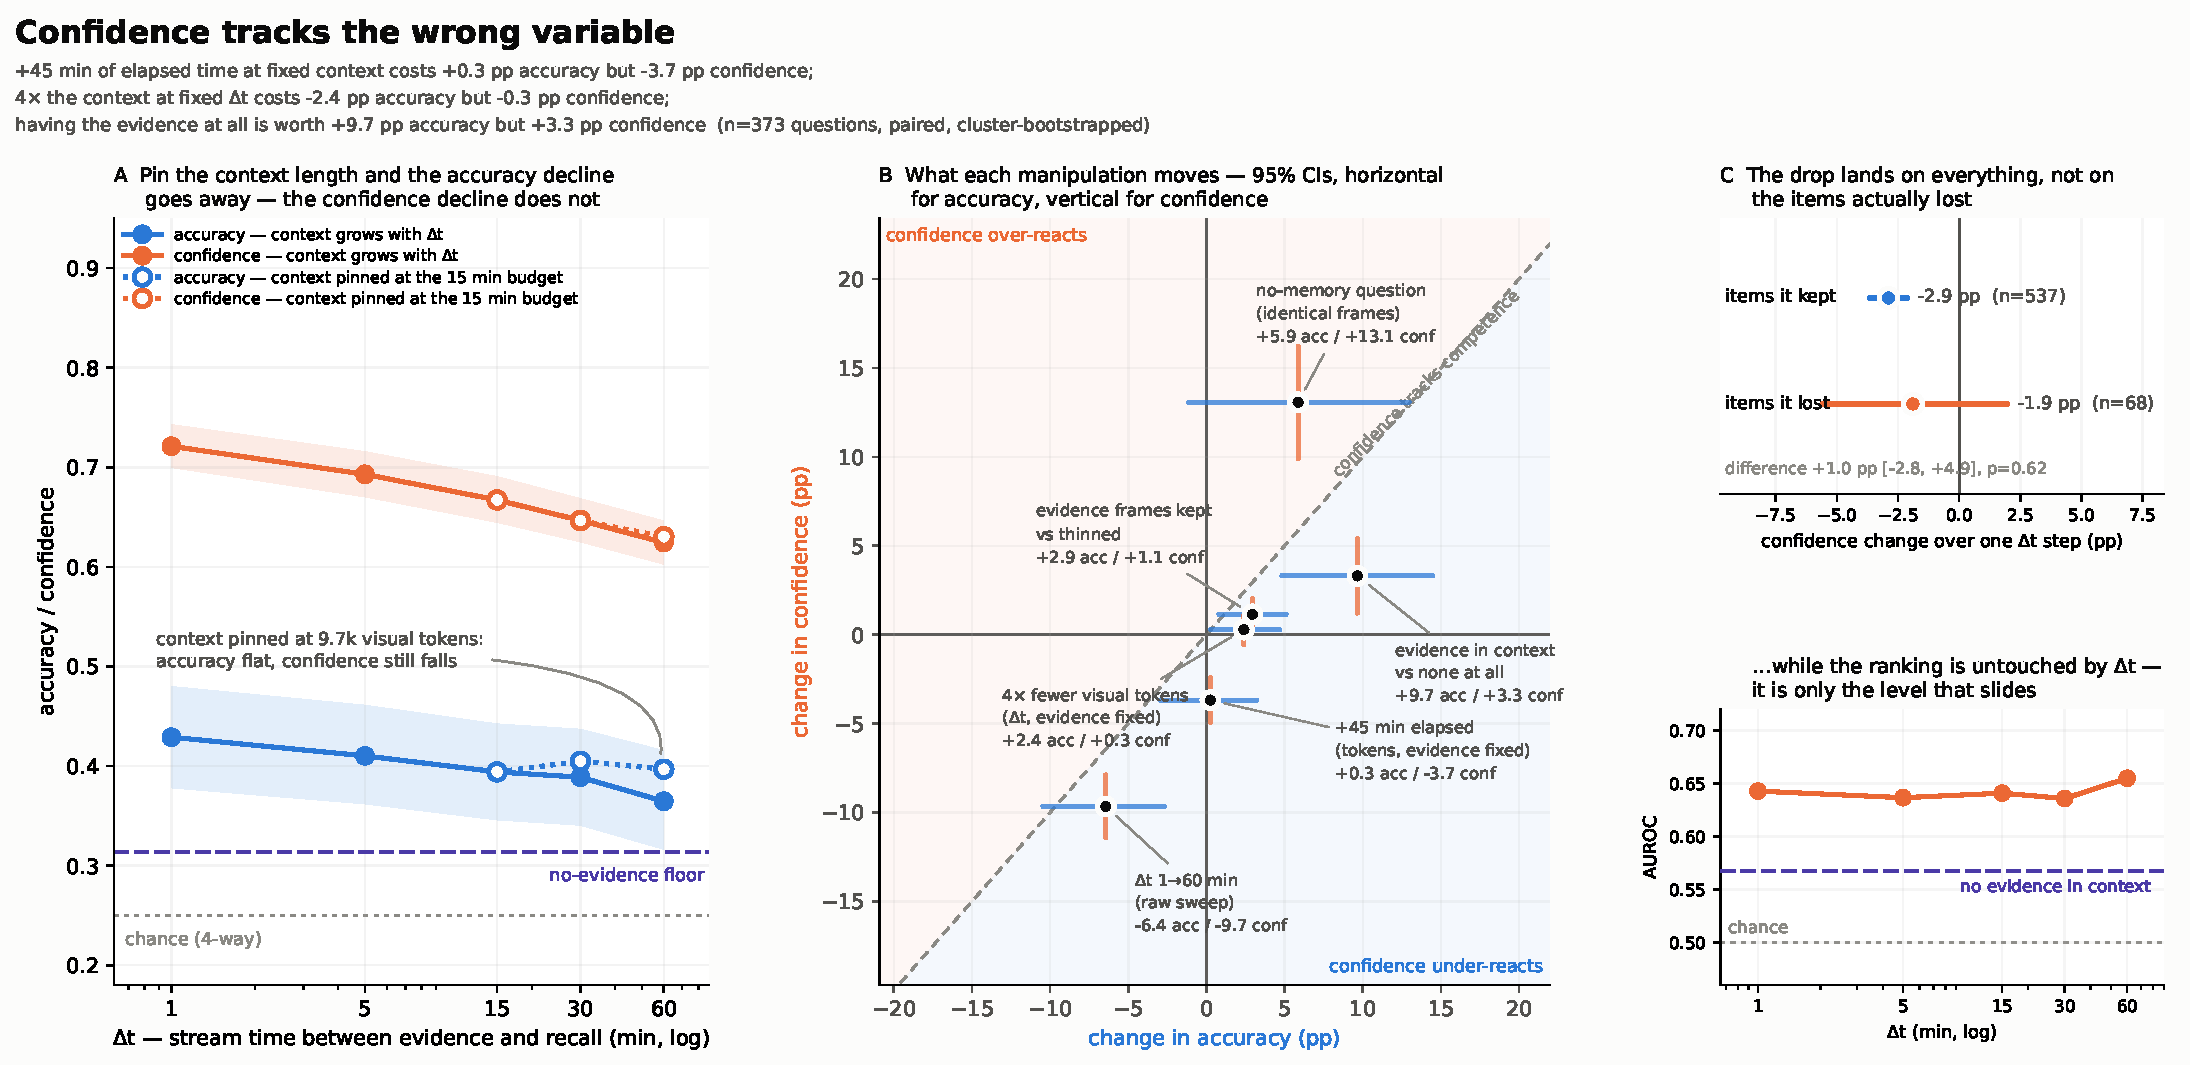
\includegraphics[width=\linewidth,height=0.68\textheight,keepaspectratio]{figures/e1-full.pdf}
    \end{column}
    \begin{column}{0.56\textwidth}
      \footnotesize
      \begin{tabular}{@{}p{2.6cm}rr@{}}
        \toprule
        \thead{manipulation} & \thead{\acc{$\Delta$acc}} & \thead{\conf{$\Delta$conf}} \\
        \midrule
        $+$45 min elapsed \newline\emph{\scriptsize(tokens fixed)} & \EoneElapsedAcc & \EoneElapsedConf \\[0.3em]
        4$\times$ fewer tokens \newline\emph{\scriptsize(\dt\ fixed)} & \EoneTokensAcc & \EoneTokensConf \\[0.3em]
        evidence vs none \newline\emph{\scriptsize(token-matched)} & \EoneEvidenceAcc & \EoneEvidenceConf \\
        \bottomrule
      \end{tabular}
      \vskip0.5em
      \claim{\scriptsize \conf{Confidence} moves on elapsed time, which costs \emph{no} accuracy. \acc{Accuracy} moves on context length and evidence, which confidence barely registers.}
    \end{column}
  \end{columns}
  \source{\texttt{figures/headline.pdf} (M7). Nothing redrawn.}
\end{frame}

\begin{frame}[t]{\Etwolong: the same dissociation, rotated}{Accuracy responds to evidence; confidence responds to context volume}
  \begin{columns}[T]
    \begin{column}{0.48\textwidth}
      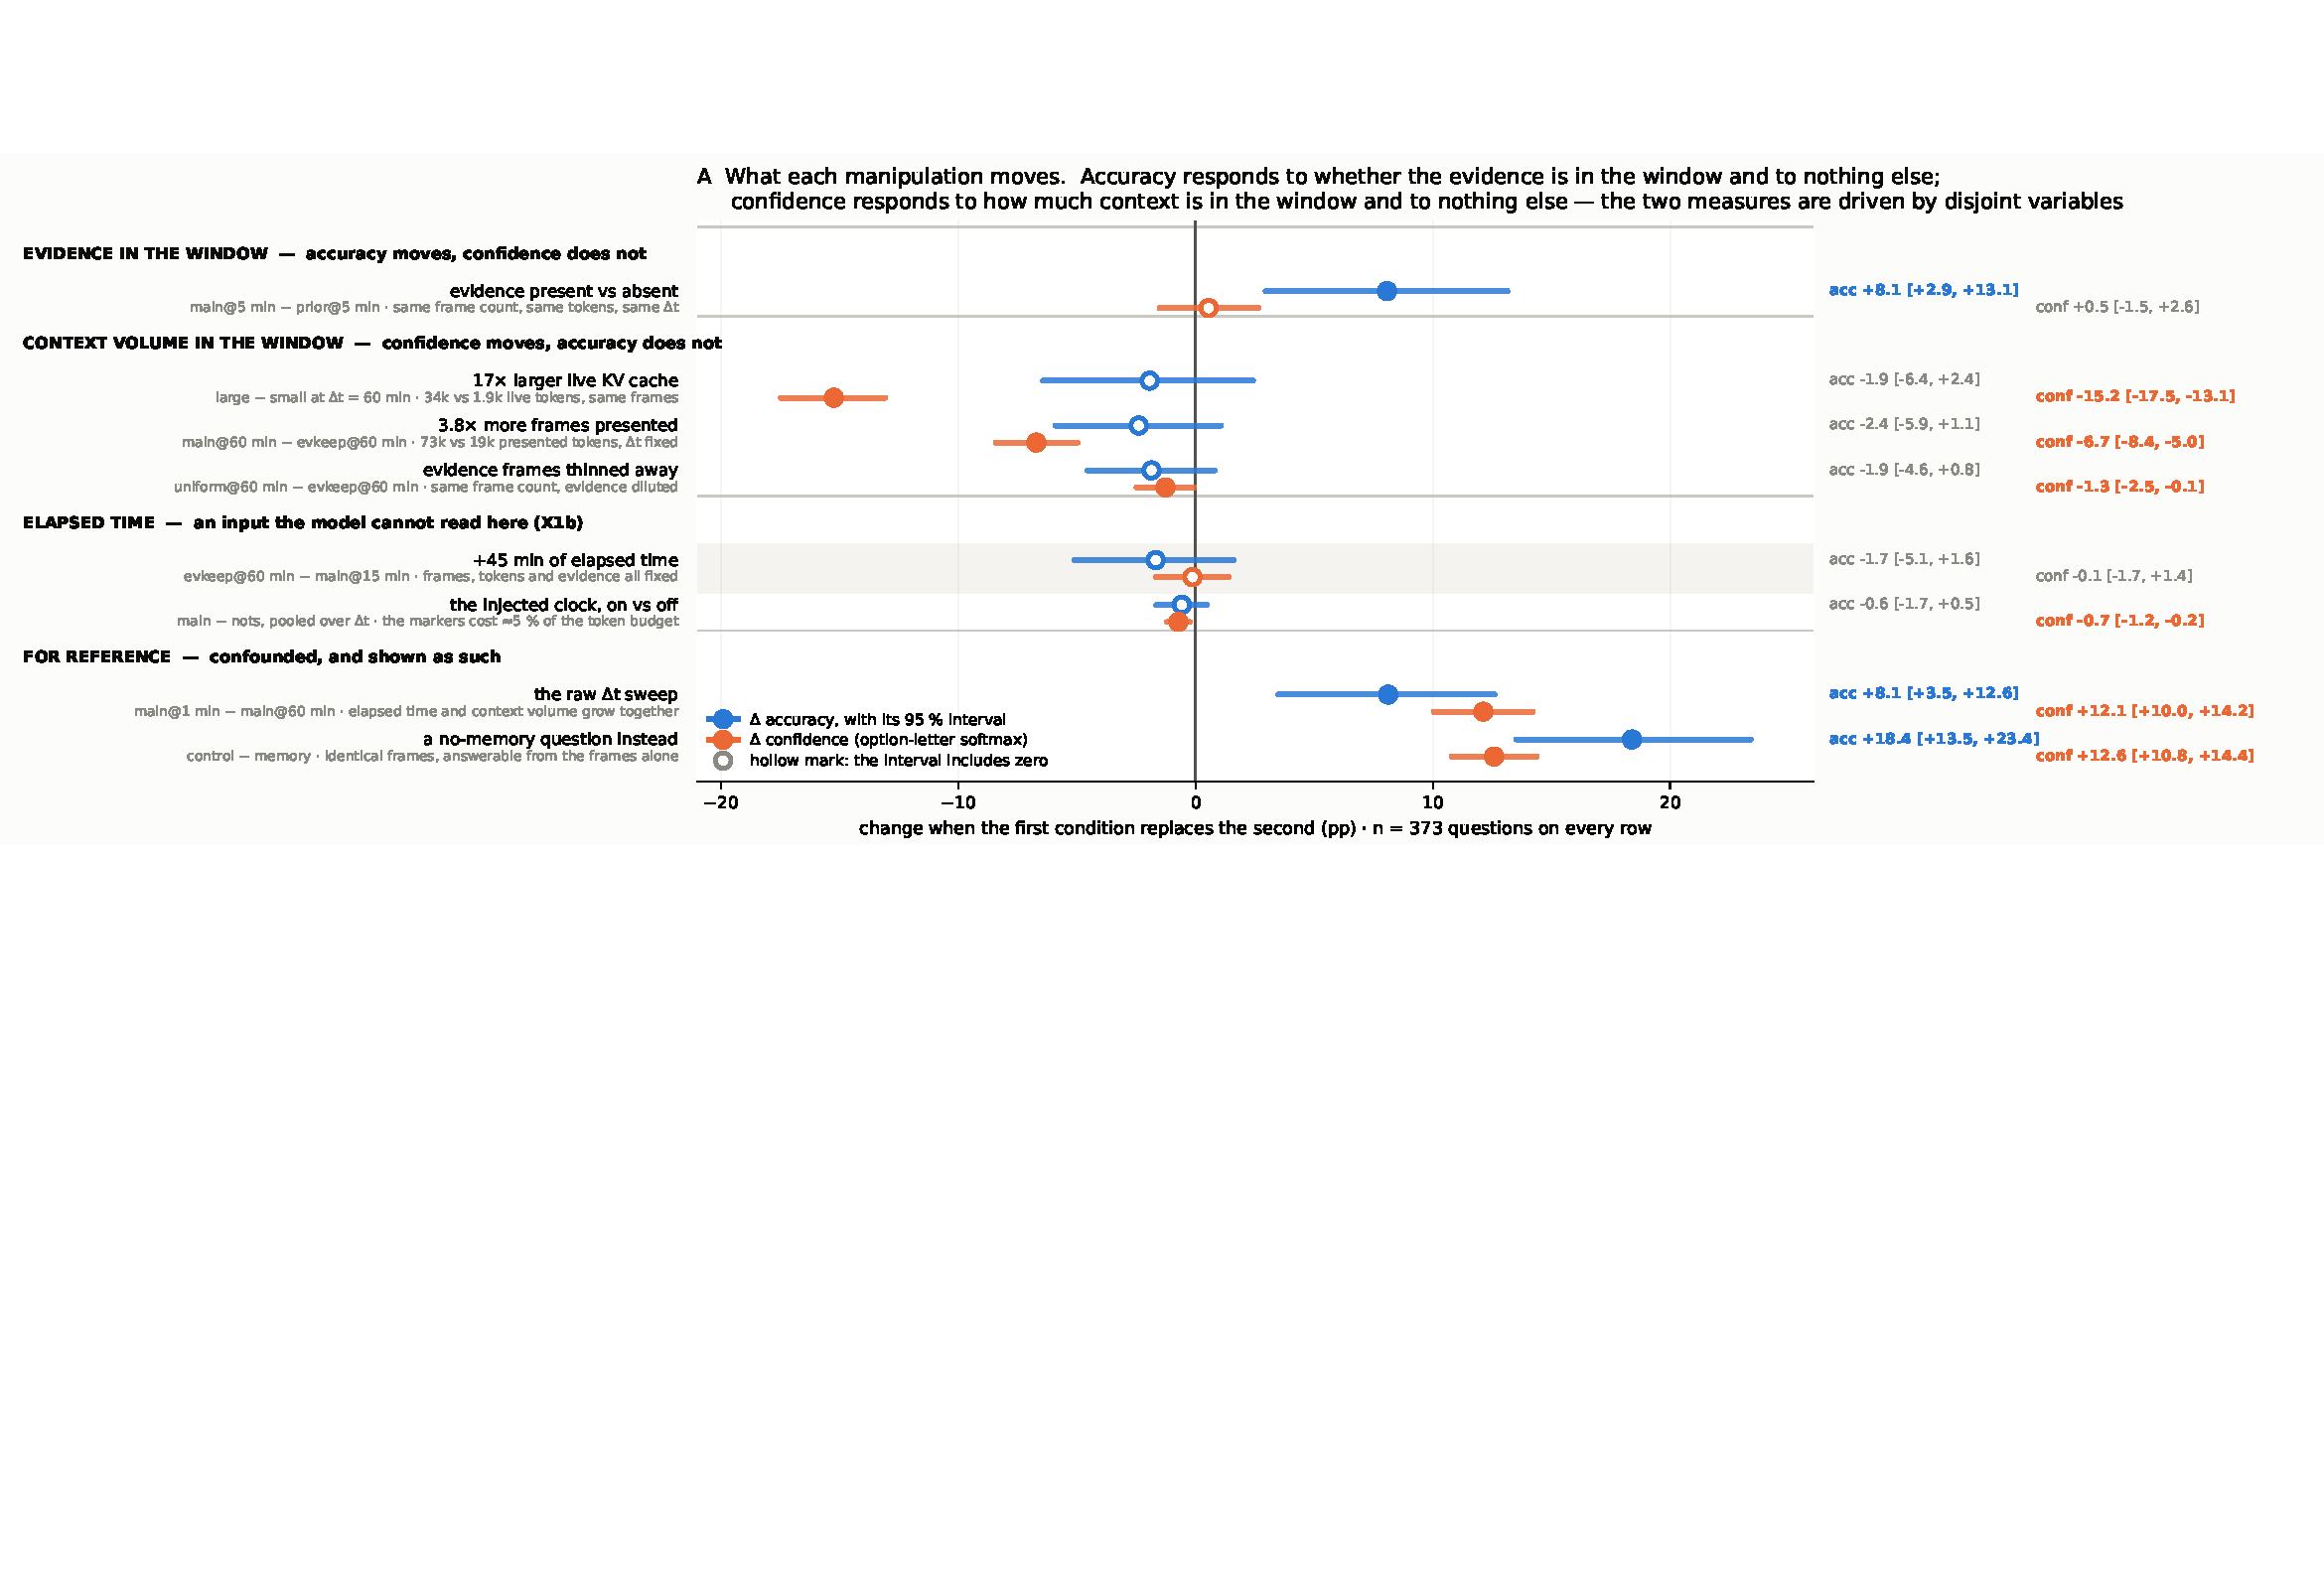
\includegraphics[width=\textwidth,height=0.62\textheight,keepaspectratio]{figures/e2-a.pdf}
      \vskip0.3em
      {\scriptsize\color{inkmid}Elapsed-time axis is \emph{unavailable}, not null --- see backup.}
    \end{column}
    \begin{column}{0.50\textwidth}
      {\footnotesize\textbf{Budget dose--response at \dt\ = 60 min:}}
      \vskip0.3em
      \scriptsize
      \begin{tabular}{@{}crr@{}}
        \toprule
        \thead{\dt\ (min)} & \thead{\acc{$\Delta$acc}} & \thead{\conf{$\Delta$conf}} \\
        \midrule
        \TabEtwoBudgetNarrow
        \bottomrule
      \end{tabular}
      \vskip0.5em
      \claim{\scriptsize A \EtwoBudgetRatio\ live-token budget is worth \acc{\EtwoBudgetAcc} of accuracy and \conf{\EtwoBudgetConf} of confidence. Monotone on one measure, flat on the other.}
    \end{column}
  \end{columns}
  \source{\texttt{figures/streaming\_headline.pdf} (X10). Full figure in backup.}
\end{frame}

\begin{frame}[t]{Cross-regime: the dissociation replicates and its driver rotates}{Differenced contrasts --- same manipulation in both regimes, paired on the same questions}
  \begin{center}\footnotesize
    \begin{tabular}{@{}p{5.2cm}rrr@{}}
      \toprule
      \thead{manipulation, $\Delta$confidence} & \thead{\Eone} & \thead{\Etwo} & \thead{difference (\Etwo\,$-$\,\Eone)} \\
      \midrule
      \TabCrossRegime
      \bottomrule
    \end{tabular}
  \end{center}
  \vskip0.5em
  \begin{columns}[T]
    \begin{column}{0.49\textwidth}
      {\footnotesize\textbf{Invariant.} Accuracy responds to evidence presence; confidence does not --- in either regime.}
    \end{column}
    \begin{column}{0.49\textwidth}
      {\footnotesize\textbf{Rotated.} In \Eone\ confidence slid with elapsed time; in \Etwo\ it slides with context volume. Both differences exclude zero.}
    \end{column}
  \end{columns}
\end{frame}

\begin{frame}[t]{Unified account and implications}
  \claim{\footnotesize\textbf{Confidence is computed from surface properties of the context} --- how much visual input was processed (retained or not), and how long ago it says that was --- \textbf{not from whether the needed information is present.} Remove one surface cue and it latches onto another. What it never latches onto is evidence.}
  \vskip0.6em
  {\footnotesize\textbf{What this does to the original claim:}}
  \begin{itemize}\footnotesize\setlength\itemsep{0.15em}
    \item \textbf{Half 1} (``widening gap as evidence ages'') --- {\color{flagred}rejected twice.}
    \item \textbf{Half 2} (``\dt-conditioned recalibration recovers reliability'') --- {\color{flagred}needs revision.} \dt\ is the wrong conditioner; it worked in \Eone\ by accident. The variable that actually drives confidence is \texttt{live\_tokens}.
    \item \textbf{Headroom differs by regime.} AUROC is flat over the \Eone\ sweep (\EoneAurocDelta) but decays in \Etwo\ (\EtwoAurocDelta, $p$ = \EtwoAurocP). Recalibrating a level only works if the ranking survives.
  \end{itemize}
  \vskip0.3em
  {\footnotesize\color{goodgreen}The cheap fix looks cheaper the less realistic the memory system is --- only visible because both regimes were run.}
\end{frame}

% B4.2 -- agenda item 2: validating the confidence probe
\setsecblurb{Should confidence be a softmax over the four option letters,\\or over the whole vocabulary? Answered on the committed records, no GPU.}
\section{Is the confidence probe the right construct?}

\begin{frame}[t]{The question, and the answer}{The alternative was already on disk --- both backends log the full-vocabulary logprobs at the letter ids}
  \begin{columns}[T]
    \begin{column}{0.52\textwidth}
      {\footnotesize With $M$ = the next-token mass on $\{$A,B,C,D$\}$, the vocabulary-normalised confidence is exactly $c_{\text{vocab}} = c_{\text{restricted}} \times M$, recoverable for every one of the \NrecEone\,+\,\NrecEtwo\ committed records at \textbf{zero GPU cost}. No re-run was needed and none was done.}
      \vskip0.9em
      {\footnotesize\textbf{Verdict: keep \texttt{max softmax(\{A,B,C,D\})} as the primary metric.}}
      \begin{itemize}\footnotesize\setlength\itemsep{0.2em}
        \item It is the \emph{coherent denominator} --- correctness is argmax over those four letters by construction, so ECE against MCQ correctness is only coherent for the restricted version.
        \item It is \emph{field-standard}, not our idiosyncrasy: EgoSAT Eq.~6 is our definition verbatim, tracing to Tsvilodub et al.\ 2024.
        \item The alternative changes nothing we report --- except one number, where it changes it for the wrong reason.
      \end{itemize}
    \end{column}
    \begin{column}{0.45\textwidth}
      \claim{\footnotesize\textbf{The design choice that actually deserves scrutiny is not the denominator.}\\[0.4em]
      It is \textbf{option-letter bias}, and a second quantity the restricted softmax throws away turns out to carry a real signal. Both are on the next slides --- and the second is the cheapest positive result available to us.}
      \vskip0.7em
      {\scriptsize\color{inkmid}Everything here was recomputed with the \emph{unchanged} contrast machinery that produced the two authoritative artifacts, so it is directly comparable to the headline numbers.}
    \end{column}
  \end{columns}
  \source{\texttt{memo/CONFIDENCE-PROBE.md}}
\end{frame}

\begin{frame}[t]{Where the choice makes no difference --- which is nearly everywhere}
  \begin{columns}[T]
    \begin{column}{0.47\textwidth}
      {\footnotesize\textbf{The model puts essentially all its mass on the letters.}}
      \vskip0.4em
      \footnotesize
      \begin{tabular}{@{}lrr@{}}
        \toprule
        & \thead{\Eone} & \thead{\Etwo} \\
        \midrule
        mean mass on $\{$A,B,C,D$\}$ & \MassEone & \MassEtwo \\
        \multicolumn{3}{@{}l}{argmax disagreements: \textbf{\ArgmaxDisagree} records} \\
        \bottomrule
      \end{tabular}
      \vskip0.5em
      {\footnotesize Prediction --- and therefore \emph{accuracy} --- is identical under the two definitions in every record we have.}
      \vskip0.8em
      {\footnotesize Every contrast in both experiments is unchanged to 0.01 pp, including the two headlines: \Etwo's context-length effect and its null on elapsed time at fixed frames.}
    \end{column}
    \begin{column}{0.50\textwidth}
      {\footnotesize\textbf{And the ranking does not care how you collapse the four-way distribution to a scalar.}}
      \vskip0.4em
      {\footnotesize AUROC against correctness, memory rows:}
      \vskip0.3em
      \footnotesize
      \begin{tabular}{@{}lrr@{}}
        \toprule
        \thead{discriminator} & \thead{\Eone} & \thead{\Etwo} \\
        \midrule
        max-p, restricted (as shipped) & \AurocRestrEone & \AurocRestrEtwo \\
        max-p, vocabulary-normalised & \AurocVocabEone & \AurocVocabEtwo \\
        negative entropy & 0.6228 & \AurocEntropyEtwo \\
        top1 $-$ top2 margin & 0.6254 & \AurocMarginEtwo \\
        \bottomrule
      \end{tabular}
      \vskip0.5em
      \claim{\footnotesize The stronger robustness statement: \textbf{however the distribution is collapsed to a scalar, the answer is the same to 2--3 decimals.} No conclusion rests on choosing max over entropy or margin.}
    \end{column}
  \end{columns}
\end{frame}

\begin{frame}[t]{The one place it does matter --- and it would silently rewrite a verdict}
  \begin{center}\footnotesize
    \begin{tabular}{@{}lrr@{}}
      \toprule
      \thead{evidence in context vs none, $\Delta$confidence} & \thead{\Eone} & \thead{\Etwo} \\
      \midrule
      restricted (as shipped) & \EoneEvidenceBoth & \RestrEvidenceEtwo \\
      vocabulary-normalised & \EoneEvidenceBoth & \VocabEvidenceEtwo \\
      \bottomrule
    \end{tabular}
  \end{center}
  \vskip0.8em
  {\footnotesize Under vocabulary normalisation \Etwo's confidence \emph{stops} being evidence-blind. Three things we have written down would change:}
  \begin{itemize}\footnotesize\setlength\itemsep{0.15em}
    \item the streaming module's verdict selector flips from \emph{``the dissociation replicates''} to \emph{``confidence tracks eviction''} --- it reads that interval's sign directly;
    \item the cross-regime claim that confidence's evidence response is \emph{weaker} under streaming (\XregEvidenceConf) loses significance;
    \item our position in the EgoSAT comparison moves from the extreme band to the middle of it.
  \end{itemize}
  \vskip0.6em
  \claim{\footnotesize\textbf{So: do not switch the denominator quietly --- it is not a cosmetic normalisation.} The fix is to make the sensitivity visible in the artifact: assert the denominator in the module, or emit both values alongside the verdict.}
\end{frame}

\begin{frame}[t]{What the flip is actually made of --- and it is a result, not a nuisance}{Implicit abstention: with a bounded cache and no evidence, the model sometimes stops wanting to emit a letter at all}
  \begin{columns}[T]
    \begin{column}{0.50\textwidth}
      {\footnotesize The effect is not a smooth rescaling --- flooring the letter mass at 0.90 removes it (\WinsorNinety). It rides on a small, heavy-tailed minority of rows:}
      \vskip0.4em
      \begin{itemize}\footnotesize\setlength\itemsep{0.15em}
        \item \HedgeRows\ carry more than 10\,\% off-letter mass;
        \item \HedgePrior\ of \emph{no-evidence} rows, against \HedgeMain\ of evidence rows;
        \item none at all at \dt\ = 30 or 60 min;
        \item in \Eone\ the maximum over every record is \HedgeEoneMax\ --- \textbf{the phenomenon does not exist there.} It is specific to the bounded cache.
      \end{itemize}
    \end{column}
    \begin{column}{0.48\textwidth}
      {\footnotesize Paired within-question, on \emph{off-letter} mass (positive = more hedging):}
      \vskip0.4em
      \footnotesize
      \begin{tabular}{@{}lr@{}}
        \toprule
        \thead{contrast} & \thead{\Etwo\ $\Delta$off-letter} \\
        \midrule
        evidence removed & \OffLetterEvidenceEtwo \\
        raw \dt\ sweep & \OffLetterSweep \\
        \bottomrule
      \end{tabular}
      \claim{\footnotesize \textbf{This converts one of \Etwo's nulls into a measured effect} --- a metacognitive signal living exactly where max-p is silent, at no GPU cost.\\[0.35em]
      Report it as \textbf{abstention}, not confidence: the two channels move in \emph{opposite} directions across \dt, and folding them lets a 1.4\,\% tail rewrite the previous slide's verdict.}
    \end{column}
  \end{columns}
\end{frame}

\begin{frame}[t]{The construct threat that is real --- option-letter bias}
  \begin{center}\footnotesize
    \begin{tabular}{@{}lll@{}}
      \toprule
      & \thead{gold letters} & \thead{what the model predicts} \\
      \midrule
      \Eone & \BiasGold & \BiasPredEone \\
      \Etwo & \BiasGold & \BiasPredEtwo \\
      \bottomrule
    \end{tabular}
  \end{center}
  \vskip0.5em
  {\footnotesize In \Eone\ that is \BiasAccEone. With \emph{no evidence in the window at all}, the model still predicts the same skewed letters at mean confidence \PriorArmConfEone\ (\Eone) and \PriorArmConfEtwo\ (\Etwo).}
  \vskip0.7em
  \begin{columns}[T]
    \begin{column}{0.48\textwidth}
      {\footnotesize\color{goodgreen}\textbf{This is good news twice over.}}
      \begin{itemize}\footnotesize\setlength\itemsep{0.15em}
        \item It is a \emph{mechanism} for evidence-blind confidence, which we currently report only phenomenologically. A content-independent option prior does not move when evidence is removed.
        \item \textbf{The paired design largely survives it.} The letter prior is a property of the question, held fixed across arms, so it differences out of every within-question contrast to first order.
      \end{itemize}
    \end{column}
    \begin{column}{0.48\textwidth}
      \claim{\footnotesize\textbf{It will be asked, and EgoSAT already runs the check we do not} (their option-order re-shuffle).\\[0.4em]
      Cheap strengthener: a \textbf{cyclic option-permutation arm} at one \dt\ bin on the evidence and no-evidence arms, averaging per-option probability across permutations before the softmax. 4$\times$ cost on a subset.}
      \vskip0.5em
      {\scriptsize\color{inkmid}It is also a further reason the level claims are weak and the contrasts are not --- which is already our stated reading.}
    \end{column}
  \end{columns}
\end{frame}

% B4.3 -- Part 3: EgoSAT (concise)
\setsecblurb{Prior art, not a scoop. It costs one novelty claim\\and independently replicates the central finding.}
\section{EgoSAT: collision and cross-validation}

\begin{frame}[t]{What EgoSAT is, and where it collides}{\EgosatCite}
  \begin{columns}[T]
    \begin{column}{0.55\textwidth}
      {\footnotesize A streaming egocentric benchmark: \EgosatScale, six tasks spanning retrospective / present / prospective, plus an answerability model and a training-free KV selection method.}
      \vskip0.5em
      {\footnotesize\textbf{Collision surface:}}
      \begin{itemize}\footnotesize\setlength\itemsep{0.1em}
        \item The confidence probe (their Eq.~6 $=$ our definition verbatim).
        \item Confidence vs temporal distance (same estimand, \EgosatLag\ vs 1--60 min).
        \item Answerability-conditioned confidence $\approx$ our evidence contrast.
        \item Online vs offline (our regime pair, but cross-model not within-backbone).
      \end{itemize}
    \end{column}
    \begin{column}{0.43\textwidth}
      \claim{\footnotesize\color{flagred}\textbf{Must fix in framing}\\[0.3em]
      \begin{itemize}\setlength\itemsep{0.15em}
        \item Drop ``first to evaluate confidence in egocentric streaming.''
        \item Attribute the probe to Tsvilodub et al.\ 2024 / EgoSAT Eq.~6.
        \item Retire ``confidently wrong'' as phrasing.
      \end{itemize}}
      \vskip0.4em
      {\scriptsize\color{inkmid}Position instead on \textbf{evidence age} and the \textbf{elapsed-time-vs-context-volume decomposition}.}
    \end{column}
  \end{columns}
\end{frame}

\begin{frame}[t]{The central finding replicates outside this lab}{Their answerability split, our evidence split --- different dataset, different backbones, same shape}
  \begin{center}\footnotesize
    \begin{tabular}{@{}lrrc@{}}
      \toprule
      \thead{model / experiment} & \thead{\acc{$\Delta$accuracy}} & \thead{\conf{$\Delta$confidence}} & \thead{under-reaction} \\
      \midrule
      Qwen2.5-VL-72B & \multicolumn{2}{c}{\EgosatSeventyTwo} & sign-flipped \\
      Qwen2.5-VL-7B & \multicolumn{2}{c}{\EgosatSevenB} & 5.7$\times$ \\
      TimeChat-Online-7B \emph{(streaming)} & \multicolumn{2}{c}{\EgosatTimeChat} & 5.6$\times$ \\
      ROI-TimeChat-Online \emph{(streaming)} & \multicolumn{2}{c}{\EgosatRoi} & 7.3$\times$ \\
      \midrule
      \textbf{ours --- \Eone} & \acc{\EoneEvidenceAcc} & \conf{\EoneEvidenceConf} & \EoneEvidenceRatio \\
      \textbf{ours --- \Etwo} & \acc{\EtwoEvidenceAcc} & \conf{\EtwoEvidenceConf} & CI through zero \\
      \bottomrule
    \end{tabular}
  \end{center}
  \vskip0.5em
  \claim{\footnotesize\color{goodgreen}\textbf{No longer a one-dataset, one-model result.} Cite as convergent evidence. Remaining differentiators: the token-matched decomposition, the within-backbone regime pair, the time scale (40--450$\times$), and the statistics.}
\end{frame}

% B4.4 -- Part 4: next steps (concise, single slide)
\setsecblurb{Proposed follow-ups ranked by what they settle per GPU-hour.}
\section{Proposed next steps}

\begin{frame}[t]{Ranked follow-ups and open decisions}
  \scriptsize
  \begin{tabular}{@{}p{3.8cm}p{1.3cm}p{9.1cm}@{}}
    \toprule
    \thead{experiment} & \thead{cost} & \thead{what it settles} \\
    \midrule
    Strip timestamps from \Eone, re-score token-matched cells & \TimestripCost &
    Whether \Eone's elapsed-time effect is a response to printed time tokens at all. \\
    Recalibrate on \texttt{live\_tokens}, per regime & free &
    The corrected Half-2 claim. AUROC asymmetry predicts success in \Eone, partial failure in \Etwo. \\
    Off-letter mass as a reported quantity & free, CPU &
    Turns the abstention signal into a result; surfaces the denominator sensitivity. \\
    Cyclic option-permutation arm, one \dt\ bin & 4$\times$, one bin &
    The option-letter bias check EgoSAT runs and this project does not. \\
    Explicit abstention (a fifth option) & $\sim$2.4 GPU-h &
    Given the words to say ``not enough information'', does the model use them? \\
    \bottomrule
  \end{tabular}
  \vskip0.7em
  {\footnotesize\textbf{Open decisions:}}
  \begin{enumerate}\footnotesize\setlength\itemsep{0.15em}
    \item Retire the original hypothesis and lead with the dissociation?
    \item Which follow-up first? (Proposed order: timestamps-off, then recalibration.)
    \item How hard to position against EgoSAT --- convergent evidence vs competing framing?
    \item Is the abstention channel worth a section, given it rides on a 1.4\,\% tail?
  \end{enumerate}
\end{frame}

% B4.9 -- backup appendix
\appendix
\setsecblurb{Raw material behind the claims.}
\section{Backup}

\begin{frame}[t]{Backup --- \Eone, the raw \dt\ sweep}
  \begin{columns}[T]
    \begin{column}{0.52\textwidth}
      \footnotesize
      \begin{tabular}{@{}crrrr@{}}
        \toprule
        \thead{\dt\ (min)} & \thead{acc \%} & \thead{conf \%} & \thead{gap} & \thead{visual tokens} \\
        \midrule
        \TabEoneSweep
        \bottomrule
      \end{tabular}
      \vskip0.5em
      {\footnotesize Bin-1 accuracy \EoneBinOneAcc\,\% sits \EoneRange\ pp above the no-evidence floor of \EoneFloorAcc\,\%. Any statement about an accuracy \emph{level} is made inside that narrow band.}
    \end{column}
    \begin{column}{0.45\textwidth}
      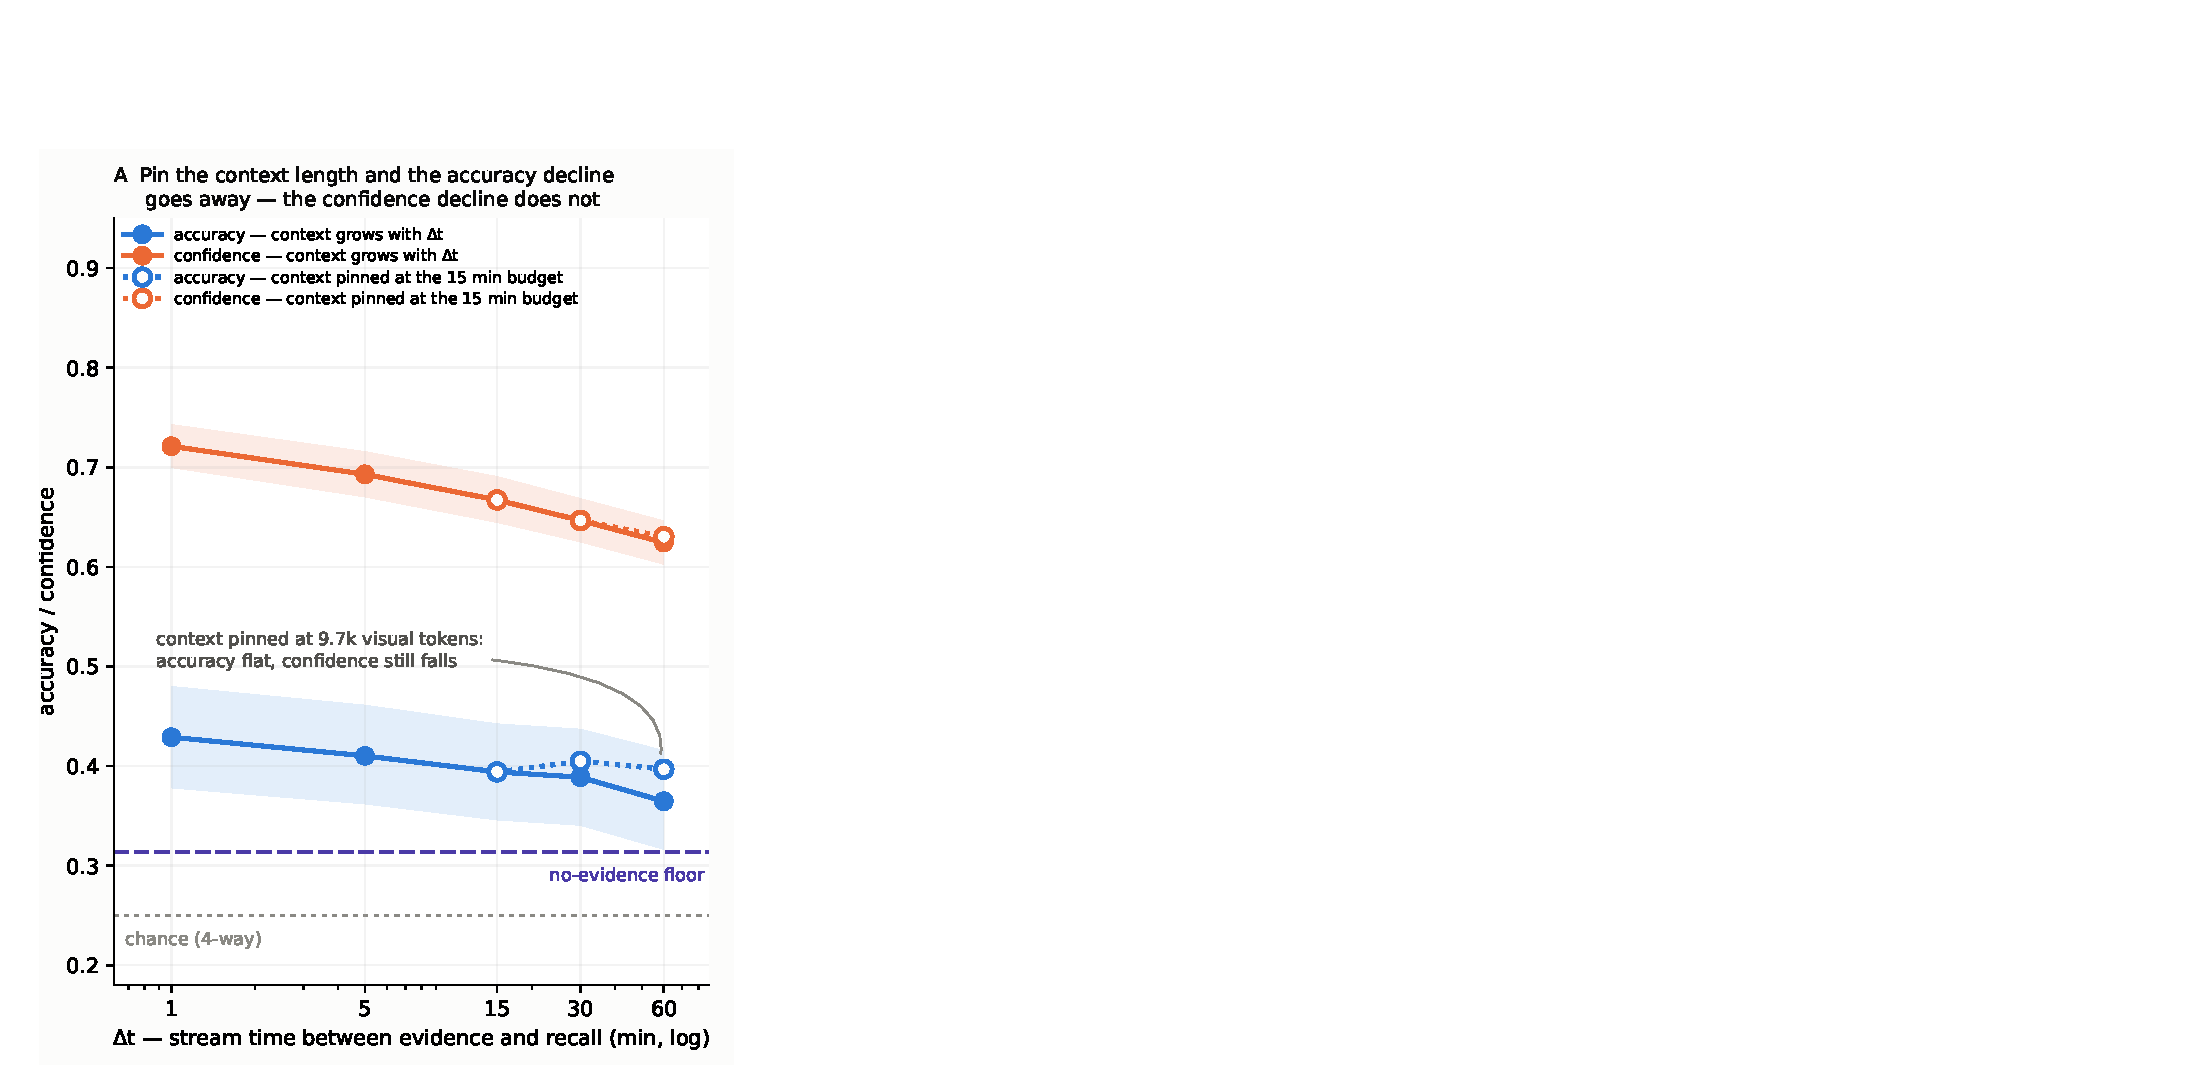
\includegraphics[width=\textwidth,height=0.72\textheight,keepaspectratio]{figures/e1-a.pdf}
    \end{column}
  \end{columns}
\end{frame}

\begin{frame}[t]{Backup --- the decomposition, in both regimes}
  \begin{columns}[T]
    \begin{column}{0.53\textwidth}
      \footnotesize
      \begin{tabular}{@{}lrr@{}}
        \toprule
        \thead{\Eone: \dt\ 15\,$\rightarrow$\,60 min} & \thead{\acc{acc}} & \thead{\conf{conf}} \\
        \midrule
        elapsed-time term & \EoneDecompAccElapsed\ pp & \EoneDecompConfElapsed\ pp \\
        context-length term & \EoneDecompAccContext\ pp & \EoneDecompConfContext\ pp \\
        \bottomrule
      \end{tabular}
      \vskip0.5em
      {\footnotesize Accuracy's decline is entirely the context term; confidence's is almost entirely elapsed time.}
      \vskip0.4em
      {\footnotesize \Etwo: \conf{\EtwoDecompConfContext\ pp} of context against \conf{\EtwoDecompConfElapsed\ pp} of elapsed time, observed \EtwoDecompConfObs\ pp, residual \EtwoDecompResid\ pp.}
    \end{column}
    \begin{column}{0.45\textwidth}
      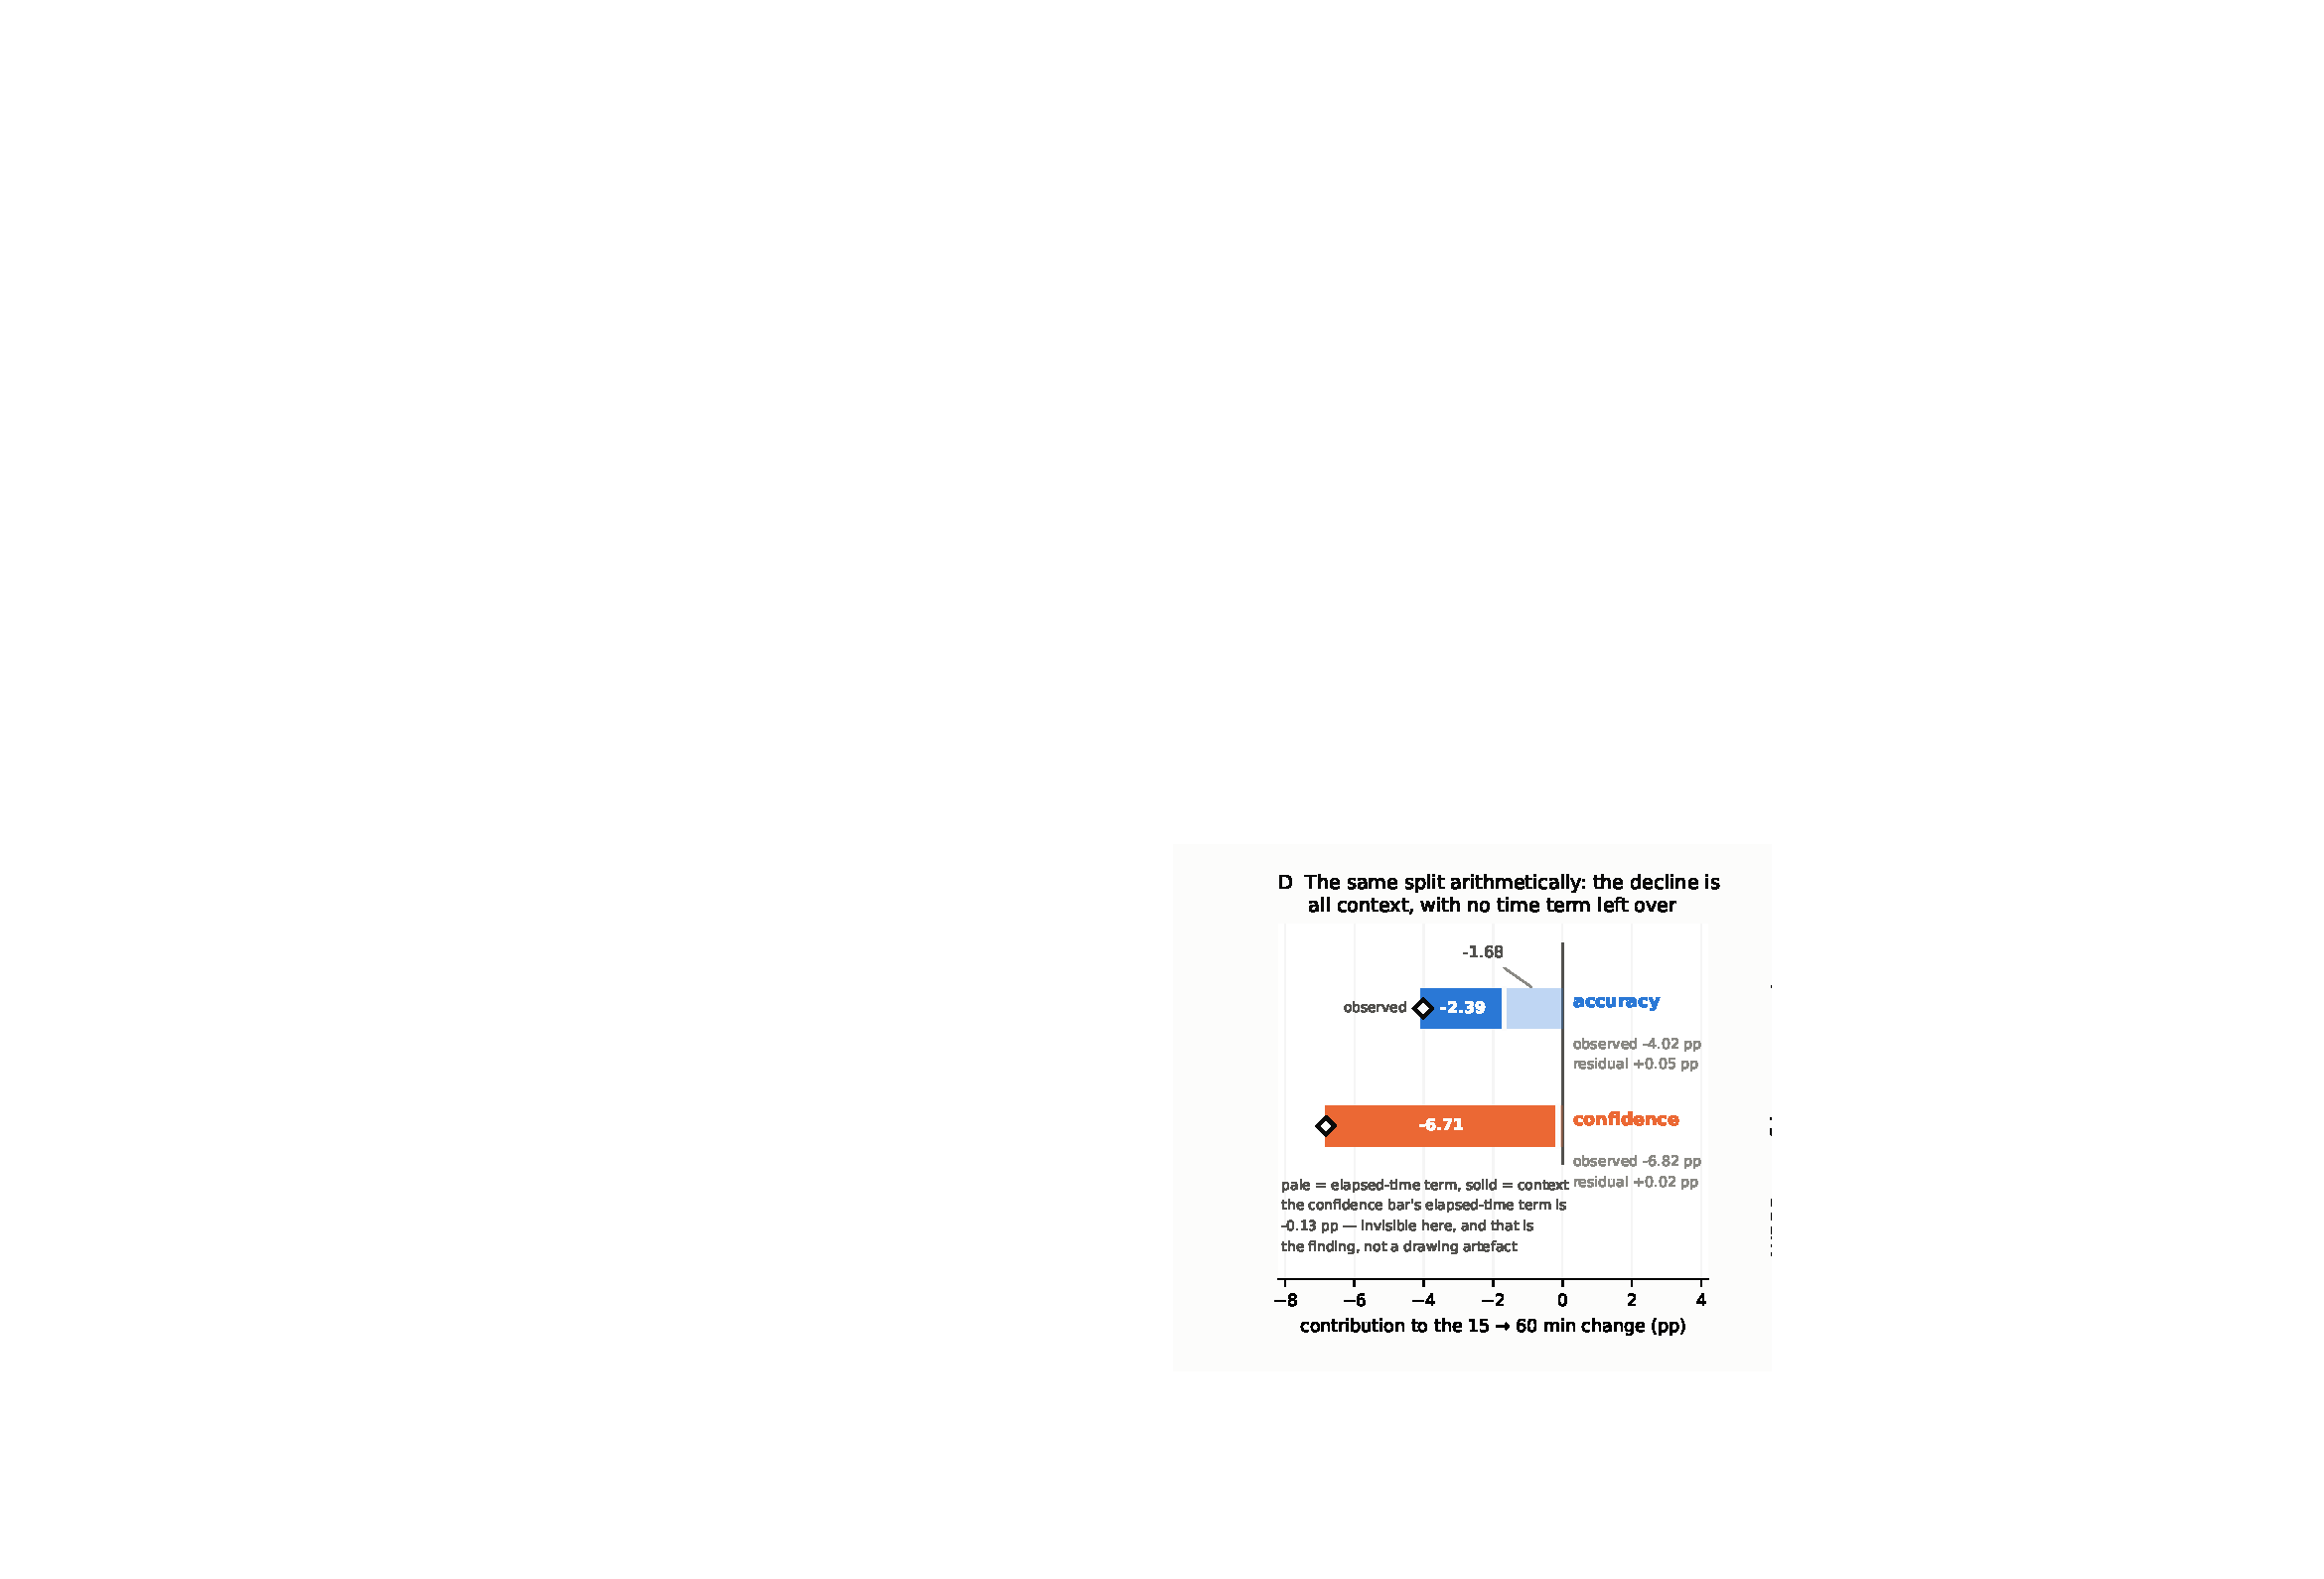
\includegraphics[width=\textwidth]{figures/e2-d.pdf}
    \end{column}
  \end{columns}
\end{frame}

\begin{frame}[t]{Backup --- \Etwo, the whole headline figure}
  \begin{center}
    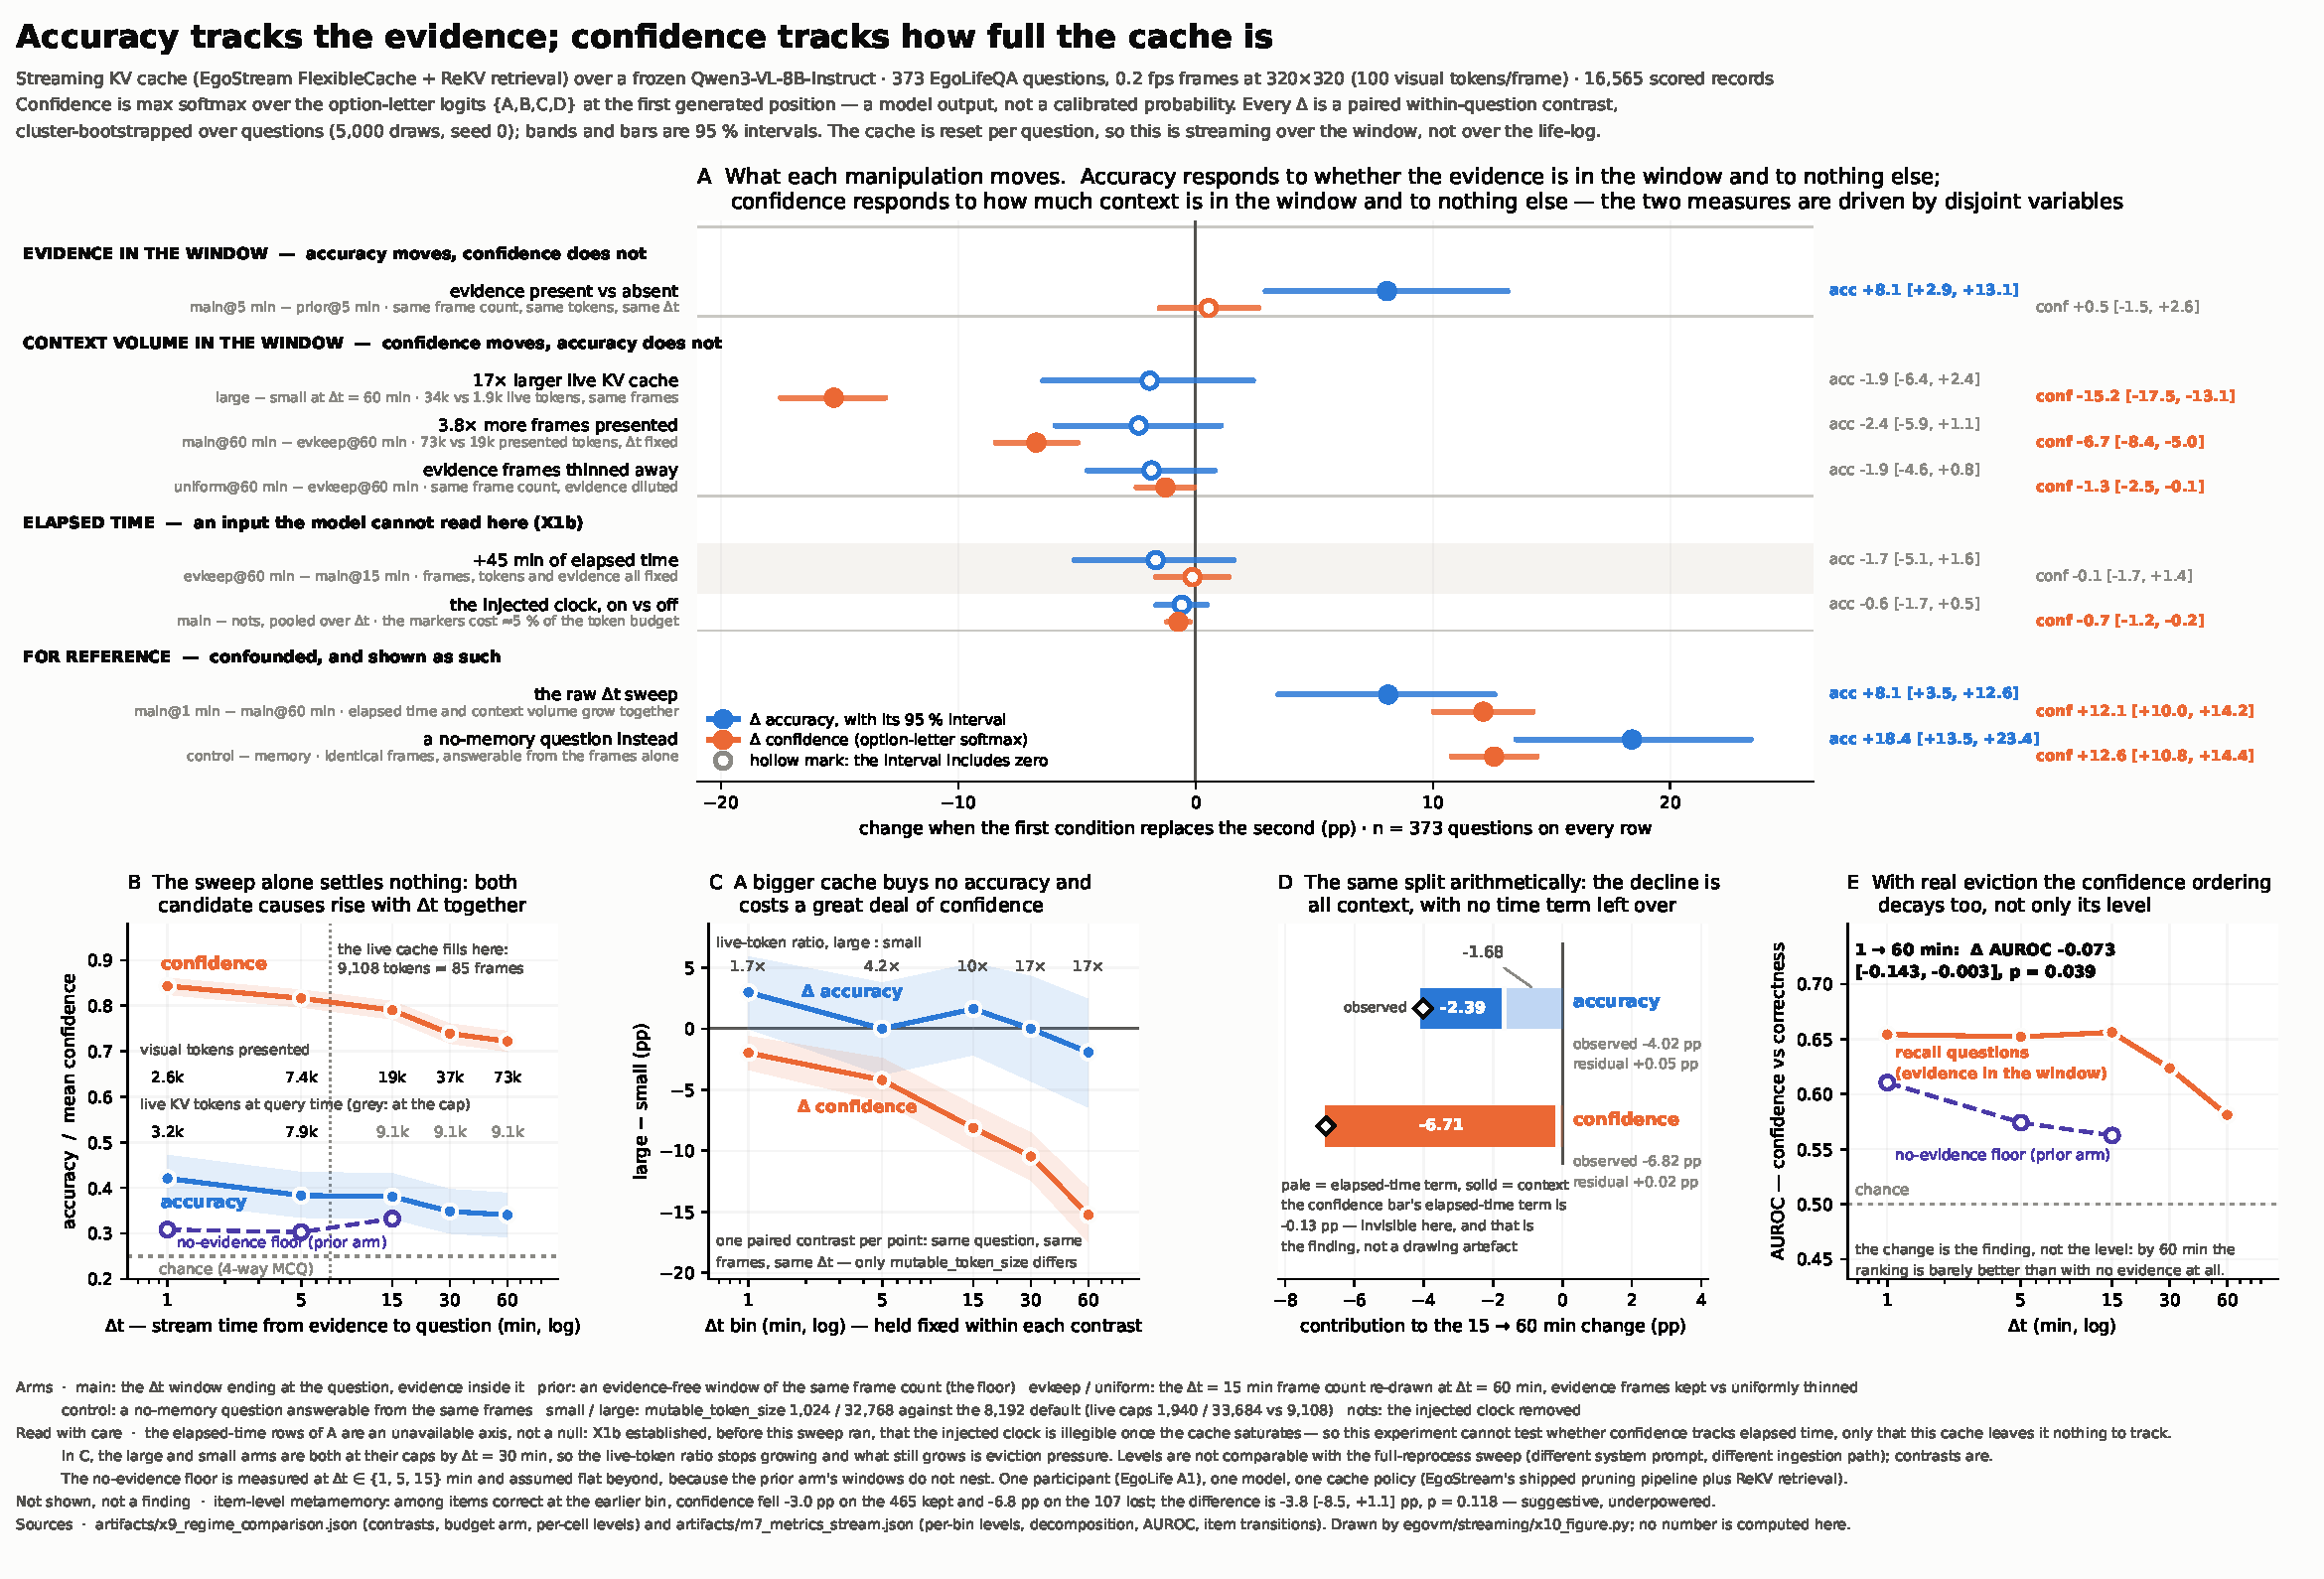
\includegraphics[width=\textwidth,height=0.80\textheight,keepaspectratio]{figures/e2-full.pdf}
  \end{center}
\end{frame}

\begin{frame}[t]{Backup --- \Etwo, full streaming contrasts}
  \begin{center}\footnotesize
    \begin{tabular}{@{}p{6.4cm}rr@{}}
      \toprule
      \thead{manipulation} & \thead{\acc{$\Delta$accuracy}} & \thead{\conf{$\Delta$confidence}} \\
      \midrule
      evidence in context vs none & \EtwoEvidenceAcc & \EtwoEvidenceConf \\
      $+$45 min elapsed, frames and evidence fixed & \EtwoElapsedAcc & \EtwoElapsedConf \\
      3.8$\times$ more presented tokens & \EtwoFourxAcc & \EtwoFourxConf \\
      \CleanBudgetRatio\ live-token budget (offload-free pair, 60 min) & \emph{\CleanBudgetAcc} & \CleanBudgetConf \\
      17$\times$ live-token budget (spans the offload boundary) & \EtwoBudgetAcc & \EtwoBudgetConf \\
      evidence frames thinned away & \EtwoThinnedAcc & \EtwoThinnedConf \\
      injected clock on vs off & \EtwoTimestampsAcc & \EtwoTimestampsConf \\
      \midrule
      raw \dt\ sweep \emph{(confounded)} & \EtwoRawAcc & \EtwoRawConf \\
      no-memory vs recall \emph{(between-items)} & \EtwoKindAcc & \EtwoKindConf \\
      \bottomrule
    \end{tabular}
  \end{center}
  \source{\texttt{artifacts/x9\_streaming.md}, generated from \texttt{x9\_regime\_comparison.json}.}
\end{frame}

\begin{frame}[t]{Backup --- three readings to rule out}
  \begin{enumerate}\footnotesize\setlength\itemsep{0.5em}
    \item \textbf{``The elapsed-time effect disappeared under streaming.''} No. EgoStream's image path carries no time markers; the injected clock is unreadable once the cache saturates. The axis is \textbf{unavailable}, not null.
    \item \textbf{``Streaming makes the model more overconfident.''} Not supported --- that is a level comparison, and the regime changes the system prompt and ingestion path. Contrasts are comparable; levels are not.
    \item \textbf{``The model tracks the items it actually lost.''} Not yet. \Etwo's kept-vs-lost difference is \EtwoItemDiff, $p$ = \EtwoItemDiffP, on \EtwoItemLost\ lost items --- suggestive, underpowered.
  \end{enumerate}
  \vskip0.4em
  \claim{\scriptsize Calling an \textbf{unavailable} axis a \textbf{null} is the most damaging misreading here --- a reviewer will make it if the paper does not pre-empt it.}
\end{frame}

\begin{frame}[t]{Backup --- where EgoSAT appears to contradict, and why it does not}
  \begin{columns}[T]
    \begin{column}{0.49\textwidth}
      {\footnotesize\textbf{1. Confidence does not fall with distance in their table} (\EgosatSixOfEight\ slopes).}
      \vskip0.3em
      {\footnotesize Against \Etwo: consistent but uninformative --- neither evidence state nor token count changes between their three probes, so their flat slope is the expected null, not a replication. Against \Eone: apparent disagreement, for three estimand differences (45 min vs 16 s; slope fitted on all-correct items only; no intervals).}
    \end{column}
    \begin{column}{0.49\textwidth}
      {\footnotesize\textbf{2. Their accuracy declines with distance} (\EgosatAccDecline\ over 8\,$\rightarrow$\,24 s) \textbf{where our token-matched arms say elapsed time costs no accuracy.}}
      \vskip0.3em
      {\footnotesize Their lag axis is uncontrolled for context volume. Their streaming models show the smallest or non-monotone declines --- matching our account.}
    \end{column}
  \end{columns}
  \vskip0.4em
  {\scriptsize The defensible framing: their uncontrolled lag axis reproduces our uncontrolled raw sweep --- and this project has the control that separates the components.}
\end{frame}

\begin{frame}[t]{Backup --- what the cache actually holds}
  \begin{columns}[T]
    \begin{column}{0.52\textwidth}
      {\footnotesize The cache: pinned priming region, evictable mutable region (the budget knob), protected hat (last two frames). On overflow, the pruning pipeline drops the lowest-value and most redundant tokens.}
      \vskip0.4em
      {\footnotesize Eviction is content-scored and global, not recency-ordered. ``Older evidence is pushed out first'' is not this policy. Eviction is permanent in the primary condition: \OffloadDefault\ default/large rows offloaded anything, against \OffloadSmall\ small rows.}
    \end{column}
    \begin{column}{0.45\textwidth}
      \claim{\scriptsize The sweep crosses saturation at \SaturationPoint. By \dt\ = 60 min only \SurvivingShare\ of the presented tokens survive, live tokens pinned at \LiveTokensIdentical\ from 15 min on.}
      \vskip0.5em
      {\scriptsize \Eone's clock is \emph{text} the model tokenizes (\EoneClockIsText), not a positional encoding --- confirmed by decoding the prompt through \Eone's own input builder.}
    \end{column}
  \end{columns}
  \source{\texttt{memo/STREAMING-CACHE.md} \S2, \S6--\S7.}
\end{frame}

\begin{frame}[t]{Backup --- dataset curation: 500 $\rightarrow$ 373 questions}
  \begin{columns}[T]
    \begin{column}{0.52\textwidth}
      \footnotesize
      \begin{tabular}{@{}p{3.8cm}rrl@{}}
        \toprule
        \thead{step} & \thead{in} & \thead{out} & \thead{reason} \\
        \midrule
        EgoLifeQA A1 (full) & 500 & --- & \\
        Drop TaskMaster & 500 & 437 & prospective \\
        Screen HabitInsight & 437 & 376 & no single anchor \\
        Evidence span $>$\,15\,min & 376 & 373 & ambiguous \dt \\
        \bottomrule
      \end{tabular}
      \vskip0.4em
      {\footnotesize\textbf{What survives.} EntityLog\,/\,EventRecall\,/\,RelationMap at 125\,/\,124\,/\,124. Answer letters 83\,:\,96\,:\,97\,:\,97. All 373 appear in every \dt\ bin and every arm; no per-bin attrition.}
      \vskip0.25em
      {\footnotesize\textbf{Token matching.} Matched arms hold visual tokens exactly at the \dt\,=\,15\,min level (mean 9,679) across all bins. Prior arms frame-matched to \texttt{main} with zero difference.}
      \vskip0.25em
      {\footnotesize\textbf{Flagged, not dropped.} \texttt{need\_audio}\,=\,true on 110/373 (29.5\,\%); results reported with and without.}
    \end{column}
    \begin{column}{0.45\textwidth}
      {\footnotesize\textbf{Why the drops are defensible.}}
      \vskip0.25em
      {\footnotesize\textbf{TaskMaster} (63): questions about future plans --- incompatible with a retrospective \dt\ sweep. 93.7\,\% require audio; the vision-only model is near-blind on them independently.}
      \vskip0.25em
      {\footnotesize\textbf{HabitInsight} (61): habitual patterns with no single evidence event to anchor \dt. Scored separately, not dropped.}
      \vskip0.25em
      {\footnotesize\textbf{Span exclusions} (3): q482 spans 50.7\,h (3 evidence points across two days; alone 13\,\% of frame-encodes). q189/q346 at 19/21\,min. Next-closest is 11.6\,min --- clean gap below the 15\,min threshold.}
      \vskip0.25em
      \claim{\scriptsize 96.5\,\% have a single evidence point (span\,=\,0). The span filter affects a small tail; ``\dt\ since evidence'' is unambiguous for the rest.}
    \end{column}
  \end{columns}
  \source{M1 \texttt{m1\_questions.py}, M4 \texttt{m4\_plan.py}; verified from \texttt{m1\_questions.jsonl} and \texttt{m4\_eval\_plan.jsonl}.}
\end{frame}

\begin{frame}[t]{Backup --- how this deck is built}
  \footnotesize
  \begin{tabular}{@{}llp{6.0cm}@{}}
    \toprule
    \thead{module} & \thead{artifact} & \thead{checks} \\
    \midrule
    B1 \texttt{b1\_numbers.py} & \texttt{generated/numbers.tex} & Re-derives all macros from metrics JSON; memo-sourced values carry a literal check. \\
    B2 \texttt{b2\_figures.py} & \texttt{figures/*.pdf} & Panels are crops; manifest pins source figures by sha256. \\
    B5 \texttt{b5\_verify.py} & the built PDF & Nine checks: stale generators, missing figures, undefined macros, LaTeX errors, overfull slides. \\
    \bottomrule
  \end{tabular}
  \vskip0.5em
  {\footnotesize No number on any slide was typed by hand. If an experiment is re-run, \texttt{make} rebuilds the deck and \texttt{make verify} fails until it is rebuilt.}
\end{frame}


\end{document}
